% !TEX encoding = UTF-8
\documentclass[a4paper,oneside,titlepage]{book}
%\usepackage[T1]{fontenc}
\usepackage[italian]{babel}

\usepackage{amsmath}
\usepackage{amssymb}
\usepackage{booktabs}
\usepackage[nouppercase]{frontespizio}
\usepackage{graphicx}
\graphicspath{{./immagini/}}
\usepackage{hyperref}
\usepackage{listings}
\usepackage{subcaption}
\usepackage{xcolor}

% Impostazioni per i listati di codice:
\definecolor{codegray}{rgb}{0.5,0.5,0.5}
\definecolor{backcolour}{rgb}{1,1,1}
\lstdefinestyle{mystyle}{
	backgroundcolor=\color{backcolour},
	numberstyle=\tiny\color{codegray},
	basicstyle=\ttfamily\footnotesize,
	breakatwhitespace=false,         
	breaklines=true,                 
	captionpos=b,                    
	keepspaces=true,
	numbersep=5pt,                  
	showspaces=false,                
	showstringspaces=false,
	showtabs=false,                  
	tabsize=2,
	mathescape
}
\lstset{style=mystyle}

% Comandi:
\newcommand{\rulesep}{\unskip\ \vrule\ }
\newcommand{\mail}[1]{\href{mailto:#1}{\texttt{#1}}}


\begin{document}

\begin{frontespizio}
	\Universita{Verona}
	\Dipartimento{Informatica}
	\Corso[Laurea]{Informatica}
	\Titolo{Riassunto del corso di Linguaggi}
	\NCandidato{Creato da}
	\Candidato{Davide Zampieri}
	\Annoaccademico{2019-2020}
\end{frontespizio}

\frontmatter
\tableofcontents

\mainmatter

% CAPITOLO 1
\chapter{Introduzione}

\section{Tipi di linguaggio}
\begin{itemize}
	\item \textit{Linguaggio matematico}: notazione molto rigorosa; può rappresentare funzioni ma non computazioni (ovvero passi di calcolo); non sempre permette rappresentazioni finite di oggetti infiniti; non sempre fornisce direttamente un metodo di calcolo di ciò che si vuole rappresentare.
	\item \textit{Linguaggio logico}: è costituito da regole di inferenza e assiomi che rendono possibile specificare il processo di computazione (ancora in modo implicito); permette di rappresentare formalmente oggetti infiniti in modo finito (ma non computazioni infinite).
	\item \textit{Linguaggio di programmazione}: permette di specificare in modo accurato esattamente le primitive del processo di computazione, con la rigorosità e la potenza della logica.
\end{itemize}

\section{Contesti di programmazione}
\begin{itemize}
	\item Applicazioni scientifiche (es. Fortran).
	\item Applicazioni economiche (es. COBOL).
	\item Intelligenza artificiale (es. LISP).
	\item Programmazione di sistemi (es. C).
	\item Web Software (es. HTML, PHP, Java).
\end{itemize}

\section{Aspetti di progettazione}
\begin{itemize}
	\item \textit{Leggibilità (Readability)}: sintassi chiara, nessuna ambiguità, facilità di lettura e comprensione dei programmi.
	\item \textit{Scrivibilità (Writability)}: facilità di utilizzo di un linguaggio per creare programmi, facilità di analisi e verifica dei programmi.
	\item \textit{Affidabilità (Reliability)}: conformità alle sue specifiche.
	\item \textit{Costo}: costo complessivo di utilizzo.
\end{itemize}

\subsection{Leggibilità}
Contribuiscono alla leggibilità:
\begin{enumerate}
	\item \textit{Semplicità}, in quanto la possibilità di poter fare la stessa cosa in più modi (es. x=x+1, x++, ...) e l'overloading degli operatori (cioè quando un singolo simbolo di operatore ha più significati) complicano i linguaggi.
	\item \textit{Ortogonalità}, in quanto più ortogonale è la progettazione di un linguaggio, meno eccezioni alle regole ci sono.
	\item \textit{Definizione dei tipi di dati}.
	\item \textit{Struttura della sintassi}.
\end{enumerate}

\subsection{Scrivibilità}
Contribuiscono alla scrivibilità:
\begin{enumerate}
	\item \textit{Semplicità e ortogonalità}.
	\item \textit{Supporto per l’astrazione}.
	\item \textit{Espressività}.
\end{enumerate}

\subsection{Affidabilità}
Contribuiscono all'affidabilità:
\begin{enumerate}
	\item \textit{Type checking}.
	\item \textit{Gestione delle eccezioni}.
	\item \textit{Assenza di aliasing}, in quanto la presenza di due o più metodi di riferimento per la stessa locazione di memoria è sicuramente un potenziale problema.
\end{enumerate}

\section{Classificazione dei linguaggi}
I linguaggi si possono classificare, per \textit{metodo di computazione}, in:
\begin{itemize}
	\item A basso livello (\textit{linguaggio binario}, \textit{Assembly}).
	\item Ad alto livello
		\begin{itemize}
			\item \textit{Linguaggi imperativi}, che descrivono come concetto chiave la cella di memoria e in cui la variabile è la sua astrazione logica che viene modificata con assegnamenti in modo sequenziale, condizionale o ripetuto.
			\item \textit{Linguaggi funzionali}, che descrivono i passi di calcolo come funzioni matematiche (compongono e applicano funzioni) e in cui le variabili non possono cambiare nel tempo.
			\item \textit{Linguaggi logici}, che usano pattern matching e unificazione/sostituzione come passo di calcolo primitivo.
		\end{itemize}
\end{itemize}
I linguaggi si possono inoltre classificare in base alle loro \textit{caratteristiche} in:
\begin{itemize}
	\item Sequenziali.
	\item Concorrenti.
	\item Modulari.
	\item Paralleli/distribuiti.
	\item Orientati agli oggetti/classi.
	\item Interpretati/scripting.
\end{itemize}

\section{Implementare linguaggi}
Un \textit{linguaggio di programmazione} \textbf{L} è un insieme di costrutti e regole per descrivere algoritmi e dati. Un \textit{programma} è un insieme finito di istruzioni/costrutti del linguaggio di programmazione.
\begin{figure}[htp]
	\begin{subfigure}{0.49\textwidth}
		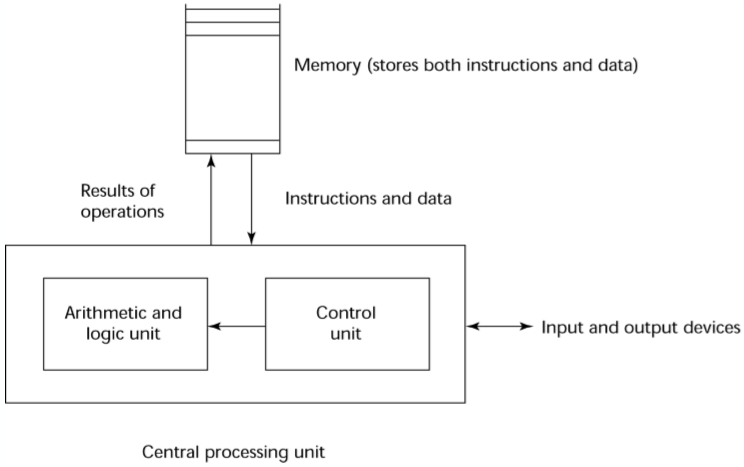
\includegraphics[width=\textwidth, height=\textheight, keepaspectratio]{vn1.png} 
		\caption{Architettura di von Neumann}
	\end{subfigure}
	\hfill
	\begin{subfigure}{0.49\textwidth}
		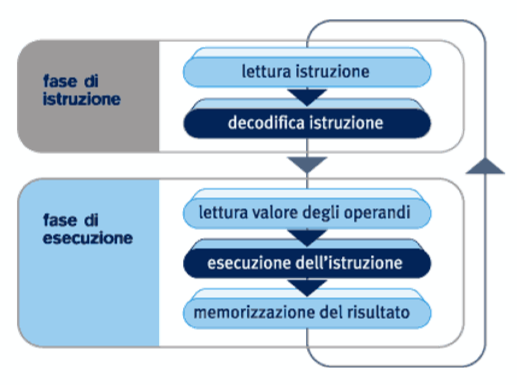
\includegraphics[width=\textwidth, height=\textheight, keepaspectratio]{vn2.png}
		\caption{Ciclo fetch-execute su una macchina di von Neumann}
	\end{subfigure}
\end{figure}

\subsection{Macchina astratta}
Implementare un linguaggio significa realizzare la \textit{macchina astratta} che interpreta il linguaggio. Dato un linguaggio \textbf{L} di programmazione, la macchina astratta \textbf{M\textsubscript{L}} per \textbf{L} è un insieme di strutture dati ed algoritmi che permettono di memorizzare ed eseguire i programmi scritti in \textbf{L}.

Quindi la macchina astratta è la combinazione di una \textit{memoria} che immagazzina i programmi e di un \textit{interprete} che esegue le istruzioni dei programmi.

Data una macchina astratta \textbf{M}, il linguaggio \textbf{L\textsubscript{M}} che ha come stringhe legali tutte le stringhe interpretabili da \textbf{M} è detto \textit{linguaggio macchina}. Infine, le macchine astratte possono essere realizzate a livello HW, FW o SW.
\begin{figure}[htp]
	\begin{subfigure}{0.49\textwidth}
		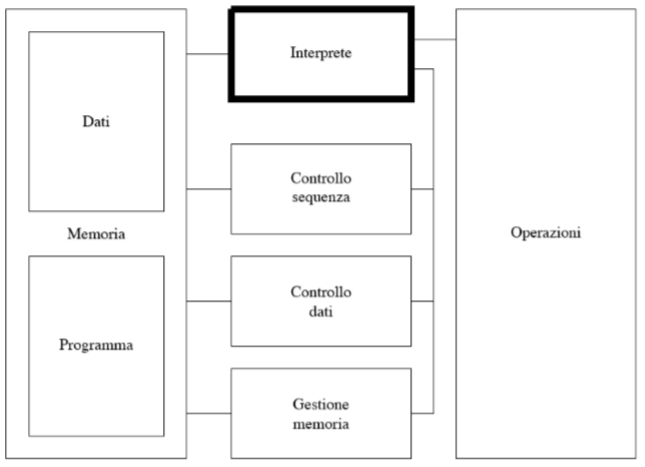
\includegraphics[width=\textwidth, height=\textheight, keepaspectratio]{ma1.png} 
		\caption{Macchina astratta}
	\end{subfigure}
	\hfill
	\begin{subfigure}{0.49\textwidth}
		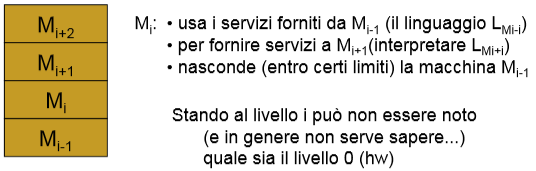
\includegraphics[width=\textwidth, height=\textheight, keepaspectratio]{ma2.png}
		\caption{Struttura a livelli cooperanti}
	\end{subfigure}
\end{figure}

\section{Come realizzare la macchina astratta}
Abbiamo un linguaggio \textbf{L} da implementare e una macchina astratta \textbf{M\textsubscript{L\textsubscript{O}}} che è la macchina ospite (con linguaggio \textbf{L\textsubscript{O}}), ovvero il livello su cui vogliamo implementare \textbf{L} e che mette a disposizione di \textbf{M\textsubscript{L}} le sue funzionalità.

Realizzare \textbf{M\textsubscript{L}} consiste quindi nel realizzare una macchina che ``traduce'' \textbf{L} in \textbf{L\textsubscript{O}}, ovvero che interpreta tutte le istruzioni di \textbf{L} come sequenza di istruzioni di \textbf{L\textsubscript{O}}. Possiamo distinguere due modalità:
\begin{itemize}
	\item \textit{Soluzione interpretativa}, cioè tramite traduzione ``implicita'' realizzata dalla simulazione dei costrutti di \textbf{M\textsubscript{L}} (ovvero di \textbf{L}) mediante programmi scritti in \textbf{L\textsubscript{O}}.
	\item \textit{Soluzione compilativa}, cioè tramite traduzione ``esplicita'' dei programmi di \textbf{L} in corrispondenti programmi di \textbf{L\textsubscript{O}}.
\end{itemize}

\subsection{Soluzione interpretativa: interprete}
Un interprete è un programma \textbf{int\textsuperscript{L\textsubscript{O},L}} che esegue, sulla macchina astratta per \textbf{L\textsubscript{O}}, il programma \textbf{P\textsuperscript{L}} con input \textbf{d $\in$ D}. Data la seguente notazione:
\begin{itemize}
	\item \textbf{Prog\textsuperscript{L}} è l'insieme di programmi scritti in \textbf{L}
	\item \textbf{D} è l'insieme di dati (input e output)
	\item Se \textbf{P\textsuperscript{L} $\in$ Prog\textsuperscript{L}} e \textbf{in,out $\in$ D} allora \textbf{[P\textsuperscript{L}]: D $\rightarrow$ D} è la semantica di \textbf{P\textsuperscript{L}} tale che \textbf{[P\textsuperscript{L}](in) = out}, ovvero se \textbf{P\textsuperscript{L}} viene eseguito a partire da \textbf{in} restituisce \textbf{out}
\end{itemize}
l'interprete \textbf{int\textsuperscript{L\textsubscript{O},L}} da \textbf{L} a \textbf{L\textsubscript{O}} è un programma tale che
\[ [int^{L_{O},L}]: (Prog^{L} \times D) \rightarrow D \]
\begin{center}
	e
\end{center}
\[ [int^{L_{O},L}](P^{L},in) = [P^{L}](in) \]
Un interprete è di fatto un ciclo che, attraverso una \textit{serie di operazioni}, esegue per simulazione le istruzioni del linguaggio.
\newpage
\noindent
Tali operazioni sono:
\begin{itemize}
	\item \textit{Elaborazione dei dati primitivi}.
	\item \textit{Controllo di sequenza delle esecuzioni} (strutture dati manipolate con operazioni specifiche).
	\item \textit{Controllo dei dati}.
	\item \textit{Controllo della memoria}.
\end{itemize}

\subsection{Soluzione compilativa: compilatore}
Un compilatore è un programma \textbf{comp\textsuperscript{L\textsubscript{O},L}} che traduce programmi scritti in \textbf{L} in programmi scritti in \textbf{L\textsubscript{O}}, e quindi eseguibili direttamente sulla macchina astratta per \textbf{L\textsubscript{O}}. Il compilatore \textbf{comp\textsuperscript{L\textsubscript{O},L}} da \textbf{L\textsubscript{O}} a \textbf{L} è un programma tale che
\[ [comp^{L_{O},L}]: Prog^{L_{O}} \rightarrow Prog^{L} \]
\begin{center}
	e
\end{center}
\[ [comp^{L_{O},L}](P^{L}) = P^{L_{O}} \text{ tale che } [P^{L_{O}}](in) = [P^{L}](in) \]
L'esecuzione di un compilatore passa attraverso varie fasi:
\begin{itemize}
	\item \textit{Analisi lessicale (scanner)}, che spezza un programma nei componenti sintattici primitivi chiamati tokens (i quali formano linguaggi regolari).
	\item \textit{Analisi sintattica (parser)}, che crea una rappresentazione ad albero della sintassi del programma dove le foglie lette da sinistra a destra costituiscono frasi ben formate del linguaggio (le quali formano linguaggi CF).
\end{itemize}

\subsection{Interprete vs Compilatore}
L'\textit{implementazione interpretativa pura} comporta:
\begin{itemize}
	\item Nessun costo di traduzione.
	\item Esecuzione lenta.
	\item Scarsa efficienza della macchina \textbf{M\textsubscript{L}}.
	\item Buona flessibilità e portabilità.
	\item Facilità di interazione a run-time (es. debugging).
\end{itemize}
L'\textit{implementazione compilativa pura} comporta:
\begin{itemize}
	\item Costi di traduzione.
	\item Esecuzione veloce.
	\item Buona efficienza.
	\item Scarsa flessibilità.
	\item Debugging più difficile.
\end{itemize}
\begin{figure}[htp]
	\begin{subfigure}{0.49\textwidth}
		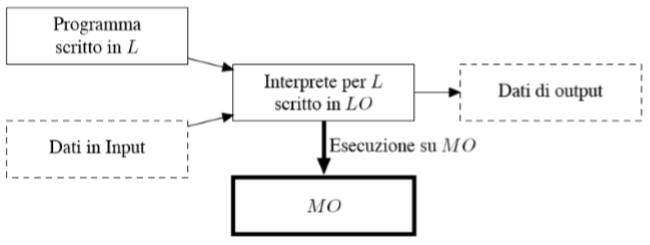
\includegraphics[width=\textwidth, height=\textheight, keepaspectratio]{int.png} 
		\caption{Implementazione interpretativa}
	\end{subfigure}
	\hfill
	\begin{subfigure}{0.49\textwidth}
		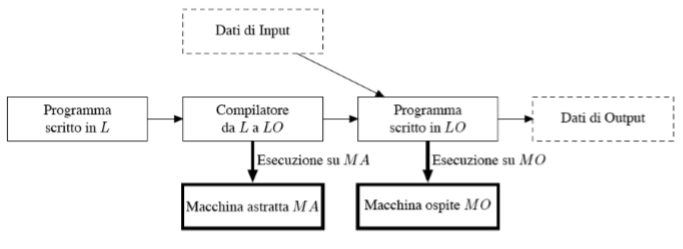
\includegraphics[width=\textwidth, height=\textheight, keepaspectratio]{comp.png}
		\caption{Implementazione compilativa}
	\end{subfigure}
\end{figure}

\subsection{Soluzione reale: ibrida}
Nella realtà, il linguaggio ad alto livello viene \textit{compilato} in un linguaggio a più basso livello che poi viene \textit{interpretato}.

Consideriamo il linguaggio \textbf{L}, ad alto livello, per il quale dobbiamo realizzare la macchina astratta \textbf{M\textsubscript{L}}: \textbf{L} viene tradotto in un linguaggio intermedio \textbf{L\textsubscript{M\textsubscript{I}}} la cui macchina astratta \textbf{M\textsubscript{I}} consiste in un interprete del linguaggio \textbf{L\textsubscript{M\textsubscript{I}}} sulla macchina ospite \textbf{M\textsubscript{O}}. 

In sintesi, nell'evoluzione dei linguaggi di programmazione esistono tre situazioni possibili:
\begin{itemize}
	\item \textit{Interprete puro}, quando \textbf{M\textsubscript{L}} = \textbf{M\textsubscript{I}} e quindi l'interprete di \textbf{L} è realizzato su \textbf{M\textsubscript{O}}.
	\item \textit{Compilatore puro}, quando la macchina intermedia \textbf{M\textsubscript{I}} è realizzata per estensione sulla macchina ospite \textbf{M\textsubscript{O}}.
	\item \textit{Implementazione mista}, quando si traducono i programmi da \textbf{L} a \textbf{L\textsubscript{M\textsubscript{I}}} e i programmi scritti in \textbf{L\textsubscript{M\textsubscript{I}}} sono interpretati su \textbf{M\textsubscript{O}}.
\end{itemize}
\begin{figure}[htp]
	\centering
	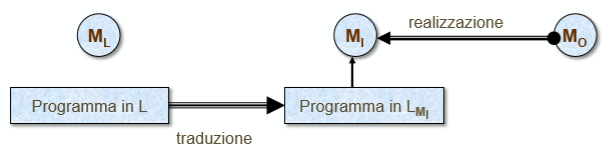
\includegraphics[width=0.9\textwidth, height=0.9\textheight, keepaspectratio]{ibrida.png}
\end{figure}

\subsection{Specializzazione}
Lo specializzatore \textit{trasforma programmi}, cioè valuta il programma su una parte dell'input, ottenendo un programma specializzato rispetto a tale input e, per questo, più efficiente. Uno specializzatore \textbf{spec\textsuperscript{L}} per \textbf{L} è un programma tale che
\[ [spec^{L}]: (Prog^{L} \times D) \rightarrow Prog^{L} \]
\begin{center}
	e
\end{center}
\[ [spec^{L}](P^{L},d) = Q^{L} \text{ tale che } [P^{L}](d,in) = [Q^{L}](in) \]
Specializzando un interprete rispetto al programma otteniamo un compilatore, in quanto: se \textbf{spec\textsuperscript{L'}} è uno specializzatore per \textbf{L'} e \textbf{int\textsuperscript{L,L\textsubscript{O}}} è un interprete da \textbf{L\textsubscript{O}} a \textbf{L} scritto in \textbf{L'}, allora \textbf{P\textsuperscript{L'} = [spec\textsuperscript{L'}](int\textsuperscript{L,L\textsubscript{O}},P\textsuperscript{L})}; infatti \textbf{P\textsuperscript{L'}} eredita l’algoritmo di \textbf{P\textsuperscript{L}} e ne esegue fedelmente le operazioni nello stesso ordine, ma con lo stile di programmazione di \textbf{int\textsuperscript{L,L\textsubscript{O}}}.


% CAPITOLO 2
\chapter{Descrivere i linguaggi}
La descrizione di un linguaggio avviene su queste \textit{dimensioni}:
\begin{itemize}
	\item Sintassi.
	\item Semantica.
	\item Pragmatica.
	\item Implementazione.
\end{itemize}

\section{Sintassi}

\subsection{Terminologia nella linguistica}
Una \textit{parola} è una stringa di caratteri su un alfabeto, mentre una \textit{frase} è una sequenza (ben formata) di parole. Un \textit{linguaggio}, quindi, è un insieme di frasi. Nell'ambito dei \textit{linguaggi di programmazione}, le parole diventano \textit{lessemi} e le frasi diventano \textit{token}. Inoltre, la frase diventa \textit{programma} quando appartiene alla categoria sintattica dei comandi.

\subsection{Descrivere la sintassi}
Nei linguaggi di programmazione, il linguaggio dei lessemi è in generale sempre un \textit{linguaggio regolare} e quindi \textit{riconosciuto} da un automa a stati finiti. Un \textit{riconoscitore}, infatti, è uno strumento di riconoscimento che legge in input stringhe sull'alfabeto del linguaggio e decide se la stringa appartiene o meno al linguaggio.

Invece, il linguaggio dei token (e dei programmi) è in generale un \textit{linguaggio context-free} (CF) e quindi \textit{generato} da una grammatica CF. Un \textit{generatore}, infatti, è uno strumento che genera stringhe di un linguaggio. Si può determinare se la sintassi di una particolare frase è sintatticamente corretta confrontandola con la struttura del generatore (parser).
\begin{figure}[htp]
	\begin{subfigure}{0.49\textwidth}
		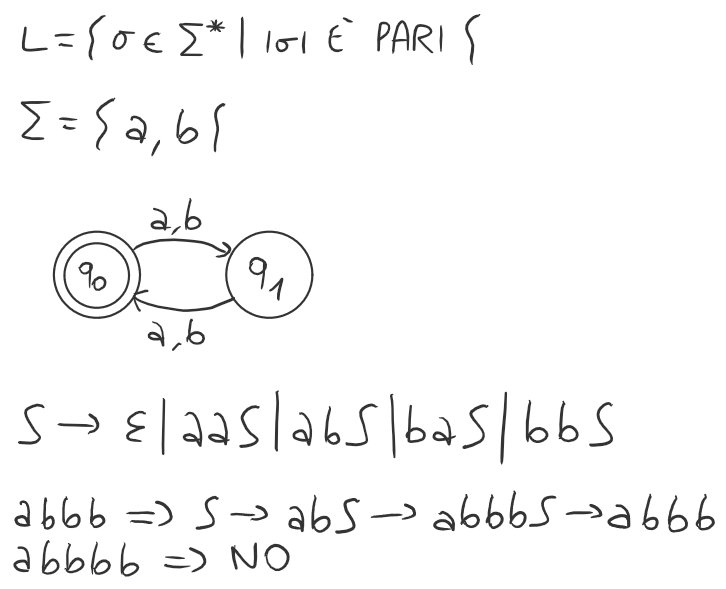
\includegraphics[width=\textwidth, height=\textheight, keepaspectratio]{automa.png} 
		\caption{Esempio di linguaggio regolare}
	\end{subfigure}
	\hfill
	\begin{subfigure}{0.49\textwidth}
		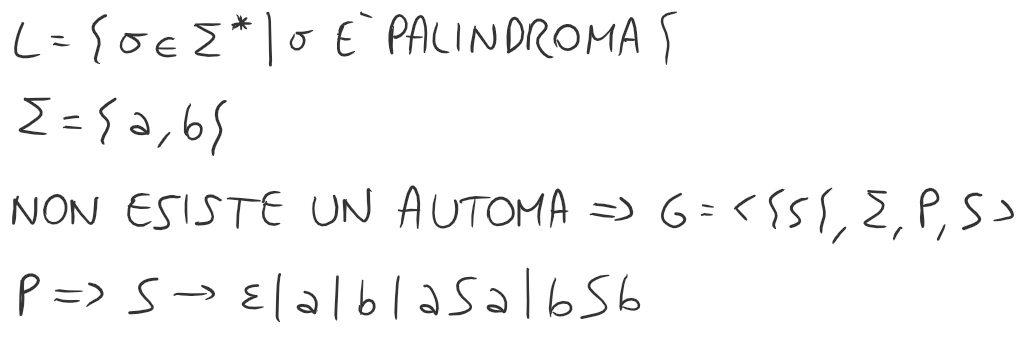
\includegraphics[width=\textwidth, height=\textheight, keepaspectratio]{grammatica.png}
		\caption{Esempio di linguaggio CF}
	\end{subfigure}
\end{figure}
\newpage

\subsection{Grammatiche context-free}
Una \textit{grammatica libera dal contesto} (CF) è una quadrupla $G = \langle V,T,P,S \rangle$ dove:
\begin{itemize}
	\item \textbf{V} è un insieme finito di variabili (dette anche simboli \textit{non terminali}).
	\item \textbf{T} è un insieme finito di simboli \textit{terminali} ($ V \cap T = \varnothing $).
	\item \textbf{P} è un insieme finito di \textit{produzioni}, in cui ogni produzione è nella forma $A \rightarrow \alpha $ dove:
	\begin{itemize}
		\item $A \in V$ è una variabile.
		\item $\alpha \in (V \cup T)^*$.
	\end{itemize}
	\item \textbf{S} è una variabile speciale detta \textit{simbolo iniziale} ($S \in V$).
\end{itemize}
Nella grammatica: i simboli non terminali sono le \textit{categorie sintattiche} (le quali rappresentano i diversi tipi di elementi che possono essere usati per comporre frasi); i simboli terminali costituiscono il \textit{vocabolario} (ovvero le parole del nostro linguaggio); le produzioni sono le \textit{regole di composizione} degli elementi in una frase; il simbolo iniziale rappresenta la \textit{categoria delle frasi} legali nel linguaggio.

\textit{Context-free} è un vincolo sulle produzioni, infatti, a sinistra possiamo trovare un solo non-terminale; ciò implica che in una frase, dovunque troviamo quel terminale, ovvero in \textit{qualunque contesto} troviamo quel terminale, lo possiamo sostituire/rimpiazzare applicando una delle produzioni per il non terminale.

Il \textit{vantaggio} delle grammatiche CF è che esistono strumenti di parsing automatici ed efficienti. Lo \textit{svantaggio} è che tali grammatiche non riescono a catturare vincoli contestuali.
\begin{figure}[htp]
	\centering
	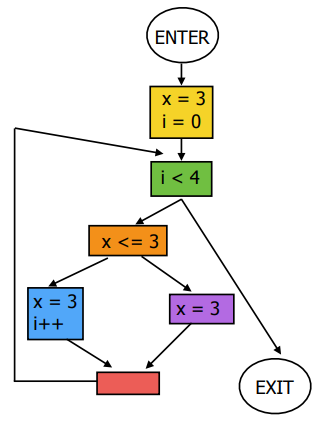
\includegraphics[width=\textwidth, height=\textheight, keepaspectratio]{cfg.png}
\end{figure}
\newpage

\subsection{Notazione BNF}
La \textit{BNF} è un metalinguaggio per descrivere linguaggi di programmazione. È stata introdotta a partire da \textit{Algol60}. Questa notazione è usata per descrivere grammatiche CF, dove: si usano intere parole come simboli terminali; i non terminali sono identificati racchiudendoli tra parentesi angolari; per le produzioni si usa il simbolo $::=$ al posto della freccia. Inoltre, esistono le seguenti \textit{opzioni}:
\begin{itemize}
	\item Parentesi quadre [ ], che indicano 0 o 1 occorrenza di quanto contenuto.
	
		\textbf{Esempio:}
		\[ <A> \, ::= \, \alpha <B> \gamma \, | \, \alpha \]
		\[ <B> \, ::= \, \epsilon \, | \, \beta_1 \, | \, \beta_2 \]
		\begin{center}
			diventa
		\end{center}
		\[ <A> \, ::= \, \alpha [\beta_1, \beta_2] \gamma \, | \, \alpha \gamma \, | \, \alpha \]
	\item Parentesi graffe \{ \}, che indicano 0 o più occorrenze di quanto contenuto.
	
		\textbf{Esempio:}
		\[ <A> \, ::= \, \alpha <B> \gamma \, | \, \alpha \]
		\[ <B> \, ::= \, \epsilon \, | \, \beta <B> \]
		\begin{center}
			diventa
		\end{center}
		\[ <A> \, ::= \, \alpha \{\beta\} \gamma \, | \, \alpha \]
\end{itemize}

\subsection{Un semplice linguaggio imperativo}
Un linguaggio può essere descritto anche in modo informale, descrivendo quali \textit{caratteristiche} vogliamo inserire e quale è il loro significato. Per esempio:
\begin{itemize}
	\item Niente dichiarazioni.
	\item Solo variabili ed espressioni booleane.
	\item Assegnamento e composizione sequenziale.
	\item Comando condizionale.
	\item Comando iterativo (loop).
\end{itemize}
Quindi, ogni linguaggio è descritto a più livelli di astrazione ognuno dei quali è a sua volta descritto da una grammatica.
\begin{figure}[htp]
	\begin{subfigure}{0.49\textwidth}
		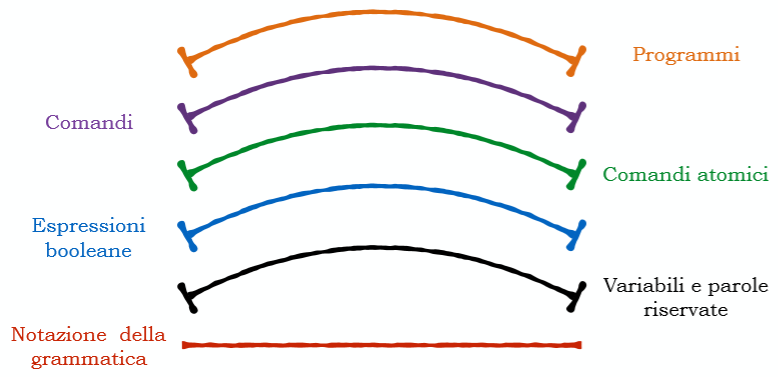
\includegraphics[width=\textwidth, height=\textheight, keepaspectratio]{imp1.png} 
		\caption{Livelli di astrazione}
	\end{subfigure}
	\hfill
	\begin{subfigure}{0.49\textwidth}
		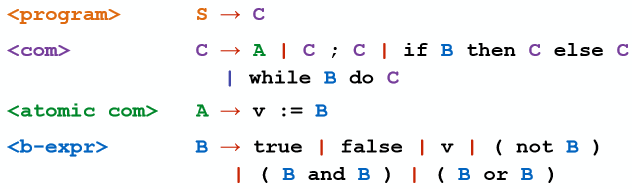
\includegraphics[width=\textwidth, height=\textheight, keepaspectratio]{imp2.png}
		\caption{Grammatiche}
	\end{subfigure}
\end{figure}

\section{Semantica}
La \textit{semantica} è più complessa della sintassi perché ricerca esattezza e flessibilità. La semantica, infatti, attribuisce un significato ad ogni frase sintatticamente corretta. I \textit{significati} sono entità autonome che esistono indipendentemente dai segni che usiamo per descriverle. La semantica del linguaggio di programmazione è anche chiamata semantica \textit{dinamica}, per distinguerla da quella \textit{statica} (cioè i vincoli semantici).  Quindi, per ogni costrutto del linguaggio va descritto il significato della sua esecuzione come trasformazione di \textit{stato}. L'astrazione della macchina nel concetto di stato permette di dare al costrutto un significato puro e indipendente dalla macchina.

\subsection{Induzione}
Abbiamo visto che la semantica va data seguendo la struttura della sintassi. La sintassi è definita descrivendo gli elementi base e componendo questi elementi (attraverso regole) in elementi composti. Questa forma di definizione ha una connotazione ben precisa nella matematica, ed è chiamata \textit{induzione}. Dato un insieme $A$ ed una relazione binaria \textbf{\textless} $\subseteq A \times A$ ben fondata (cioè senza catene discendenti infinite):
\begin{itemize}
	\item Se $A = \mathbb{N}$ si ha \textit{induzione matematica}.
	\item Se $A = L(G)$, dove $L(G)$ è un linguaggio generato da una grammatica $G$, si ha \textit{induzione strutturale}.
\end{itemize}
Secondo il \textit{principio di induzione strutturale}, per dimostrare che una proprietà è valida per tutti gli elementi di una categoria sintattica, per prima cosa si dimostra la proprietà per tutti gli \textit{elementi base} della categoria (base induttiva), e poi si dimostra la proprietà per tutti gli \textit{elementi composti} assumendo che la proprietà sia verificata da tutti i loro componenti immediati (ipotesi induttiva).
\begin{figure}[htp]
	\centering
	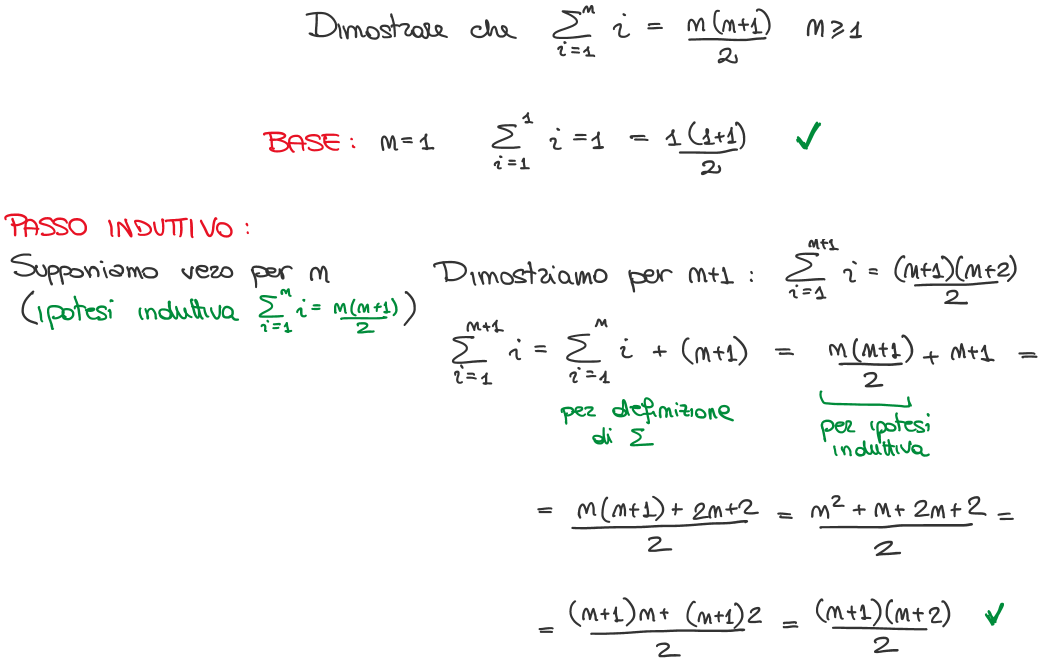
\includegraphics[width=\textwidth, height=\textheight, keepaspectratio]{induzione.png}
\end{figure}

\subsection{Descrivere i significati}
Per capire come la semantica descrive il significato, dobbiamo utilizzare i seguenti \textit{punti di vista}:
\begin{itemize}
	\item \textit{Comportamento I/O}, che interessa l'implementatore.
	\item \textit{Funzione descritta dall'algoritmo}, che interessa il progettista.
	\item \textit{Proprietà invarianti}, che interessa lo sviluppatore.
\end{itemize}
Quindi, a seconda di quali strumenti matematici usiamo per descrivere i significati, otteniamo tipi di semantiche diverse:
\begin{itemize}
	\item \textit{Semantica denotazionale}, che descrive funzionalità.
	\item \textit{Semantica assiomatica}, che descrive proprietà.
	\item \textit{Semantica operazionale}, che descrive trasformazioni di stato.
\end{itemize}

\subsection{Semantica denotazionale}
Si tratta di un modello matematico basato sulla \textit{ricorsione}, ed è la semantica più ``\textit{astratta}'' con cui descrivere i programmi. Il processo di costruzione della semantica denotazionale per un linguaggio consiste nel definire un oggetto matematico per ogni entità del linguaggio e nel definire poi una \textit{funzione} che mappa istanze delle entità del linguaggio in istanze dei corrispondenti oggetti matematici. Formalmente, il modello matematico usato per descrivere la semantica denotazionale è quello delle funzioni matematiche (ricorsive), ovvero un programma corrisponde ad una funzione del tipo
\[ E: Prog \rightarrow ((Var \rightarrow Val) \rightarrow (Var \rightarrow Val)) \]
e l'\textit{equivalenza di programmi} si dimostra mediante \textit{uguaglianza tra funzioni}.
\begin{figure}[htp]
	\centering
	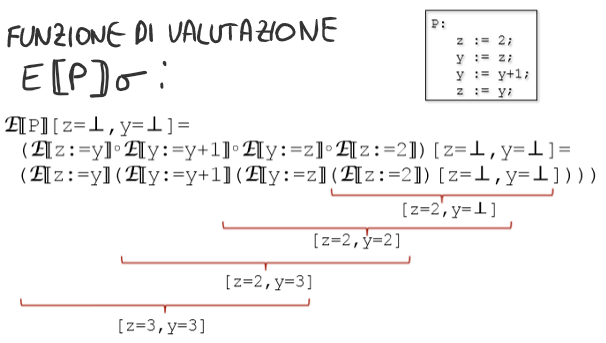
\includegraphics[width=0.7\textwidth, height=0.7\textheight, keepaspectratio]{denotazionale.png}
\end{figure}

\subsection{Semantica assiomatica}
Si tratta di un modello matematico basato sulla \textit{logica formale} (calcolo dei predicati). La semantica assiomatica, infatti, nasce con l'obiettivo di fare \textit{verifica formale di programmi}. Le espressioni logiche della semantica sono chiamate \textit{asserzioni}, le quali possono essere:
\begin{itemize}
	\item \textit{Precondizioni}, cioè asserzioni che precedono un comando e che dichiarano le relazioni e i vincoli validi prima dell'esecuzione del comando stesso.
	\item \textit{Postcondizioni}, cioè asserzioni che seguono il comando.
	\item \textit{Weakest precondition}, cioè la precondizione meno restrittiva che garantisce la postcondizione.
\end{itemize}
\begin{figure}[htp]
	\centering
	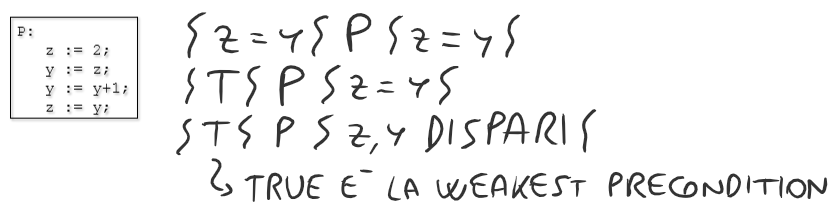
\includegraphics[width=0.7\textwidth, height=0.7\textheight, keepaspectratio]{assiomatica.png}
\end{figure}

\subsection{Semantica operazionale}
Si tratta di un modello matematico basato sui \textit{sistemi di transizione} (come i risultati finali vengono calcolati). La semantica operazionale, infatti, descrive il significato dei programmi come \textit{trasformazioni di stato}.
\\
Si consideri la funzione \textit{memoria} $\sigma: Var \rightarrow Val$ che associa valori alle variabili. Lo \textit{stato} è una coppia $<P,\sigma>$ che consiste nel programma ancora da eseguire e nello stato in cui si deve eseguire il programma. Ad ogni passo si esegue un'operazione e si cambia stato applicando una \textit{relazione tra stati} (o relazione di transizione) $\rightarrow \subseteq <P,\sigma> \times <P,\sigma>$. Tale semantica opera eseguendo i comandi separati da \textbf{;} sequenzialmente e nell'ordine in cui compaiono da sinistra a destra.
\begin{figure}[htp]
	\centering
	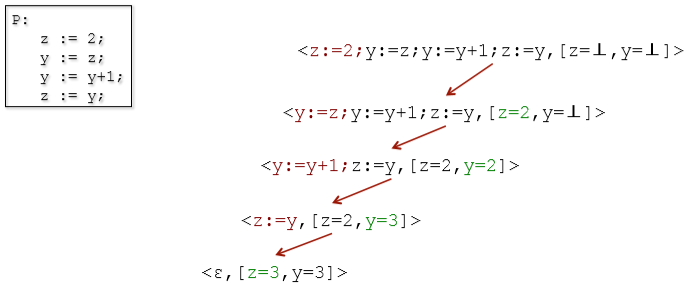
\includegraphics[width=0.7\textwidth, height=0.7\textheight, keepaspectratio]{operazionale.png}
\end{figure}

\subsection{Composizionalità}
La composizionalità è una \textit{proprietà} della semantica necessaria per caratterizzare i comportamenti e i significati di sistemi che possono avere infiniti elementi. Si noti che la semantica \textit{denotazionale} e la semantica \textit{assiomatica} rispettano banalmente tale principio. La composizionalità della semantica \textit{operazionale} è invece meno immediata.

Tale proprietà dice che il significato di ogni programma deve essere funzione del significato dei costituenti immediati. Infatti, se la semantica su cui si basa una analisi è composizionale, allora è possibile analizzare il software separatamente nei suoi moduli, per poi ricomporre il risultato dell'analisi componendo i risultati ottenuti sui singoli moduli.

\subsection{Equivalenza}
Due programmi sono equivalenti quando hanno la \textit{stessa semantica} (funzionalità, esecuzione, proprietà). L'equivalenza serve a varie \textit{fasi di analisi}:
\begin{itemize}
	\item \textit{Correttezza}, per dimostrare che il programma scritto calcola esattamente quella funzione.
	\item \textit{Equivalenza di programmi}, per dimostrare che due programmi calcolano la stessa funzione.
	\item \textit{Efficienza}, per dimostrare quale tra due programmi che calcolano la stessa funzione lo fa in modo più efficiente.
\end{itemize}

\section{Categorie sintattiche}
Dal punto di vista formale, le categorie sintattiche sono i simboli \textit{non terminali} della grammatica e servono per classificare i costrutti in funzione del loro significato atteso, ovvero della classe di effetti che la loro esecuzione causa.
\\
Possiamo identificare tre fondamentali \textit{effetti} derivanti dall'esecuzione di un programma: generazione di \textit{valori}; creazione di \textit{legami}; trasformazioni di \textit{stato}.

Le categorie sintattiche necessarie per parlare di linguaggi di programmazione si distinguono in funzione di cosa denotano/producono/ottengono rispetto ad uno stato di computazione. Partendo da questo otteniamo esattamente tre \textit{categorie}: espressioni, comandi e dichiarazioni.

\subsection{Stato}
Lo \textit{stato} è composto da due entità: ambiente e memoria. L'\textit{ambiente} (environment) è l'insieme dei legami (bindings) tra identificatori e denotazioni. La \textit{memoria} (store) è l'insieme degli effetti sugli identificatori (causati dagli assegnamenti). Quindi, l'ambiente specifica quali nomi sono usati e per quali oggetti, mentre la memoria fornisce un binding tra locazione e valore.

\subsection{Espressioni}
Le espressioni \textit{denotano valori} e devono essere \textit{valutate} per restituire un valore. Due espressioni sono \textit{equivalenti} se vengono valutate nello stesso valore in tutti gli stati di computazione (anche eventuali side-effects devono essere gli stessi). Ad esempio, \textbf{not(a and b)} è logicamente equivalente a \textbf{(not a) or (not b)} anche se le due espressioni sono sintatticamente diverse.

\subsection{Dichiarazioni}
Le dichiarazioni \textit{denotano richieste di modifica/creazione di legami} associati agli identificatori, ovvero gli ambienti. Le dichiarazioni devono essere \textit{elaborate} per attuare le modifiche agli ambienti, che sono \textit{trasformazioni reversibili}. Due dichiarazioni sono \textit{equivalenti} se producono lo stesso ambiente (e la stessa memoria in caso di side-effects) in tutti gli stati di computazione.

\subsection{Comandi}
I comandi \textit{denotano richieste di modifica della memoria}. I comandi rappresentano funzioni di trasformazione e devono essere \textit{eseguiti} per attuare le modifiche della memoria, che sono \textit{trasformazioni irreversibili}. Due comandi sono \textit{equivalenti} se per ogni stato (memoria) in input producono lo stesso stato (memoria) in output.

\subsection{Riassunto}
Le \textit{categorie sintattiche} dei linguaggi di programmazione sono:
\begin{itemize}
	\item \textit{Espressioni}, che vengono valutate in valori e non modificano lo stato di computazione e gli ambienti.
	\item \textit{Dichiarazioni}, che vengono elaborate per creare/modificare ambienti/legami (modifiche reversibili) e non producono valori né modificano la memoria.
	\item \textit{Comandi}, che eseguono modifiche irreversibili della memoria e non producono valori né modificano ambienti.
\end{itemize}

\section{Sistemi di transizione}
La semantica deve essere \textit{specificata} in funzione della sintassi. Il modo migliore per descrivere la semantica è attraverso la \textit{manipolazione di simboli}. Lo strumento formale utilizzato è quello dei \textit{sistemi di transizione}, i quali hanno le seguenti caratteristiche:
\begin{itemize}
	\item Sono \textit{matematicamente precisi}.
	\item Sono molto \textit{concisi}.
	\item Sono un \textit{metodo di specifica generale} che permette \textit{astrazione}.
	\item Sono espressi mediante una \textit{collezione di regole} date in funzione della sintassi (\textit{induttivamente}), cioè \textit{specificano cosa viene calcolato} tramite induzione sulla struttura sintattica del linguaggio.
\end{itemize}
Per definizione, un sistema di transizione è una struttura $(\Gamma,\rightarrow)$, dove $\Gamma$ è un insieme di elementi $\gamma$ chiamati \textit{configurazioni} e la relazione binaria $\rightarrow \subseteq \Gamma \times \Gamma$ è chiamata \textit{relazione di transizione}. Se $T \subseteq \Gamma$ è un insieme di configurazioni terminali, il sistema è detto \textit{terminale}.
\begin{figure}[htp]
	\begin{subfigure}{0.49\textwidth}
		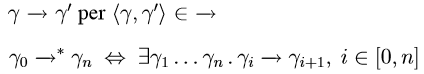
\includegraphics[width=\textwidth, height=\textheight, keepaspectratio]{sdt1.png} 
		\caption{Notazione}
	\end{subfigure}
	\hfill
	\begin{subfigure}{0.49\textwidth}
		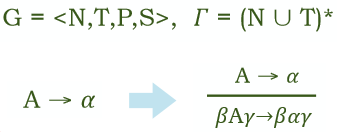
\includegraphics[width=\textwidth, height=\textheight, keepaspectratio]{sdt2.png}
		\caption{Generazione di $(\Gamma,\rightarrow)$ a partire da una grammatica CF}
	\end{subfigure}
\end{figure}

\section{PL0 - un semplice linguaggio reale}
Le \textit{caratteristiche} di PL0 (un linguaggio \textit{Pascal-like}) sono:
\begin{itemize}
	\item \textit{Singolo tipo di dato} INTEGER (i Booleani vengono rappresentati come interi).
	\item \textit{Strutture di controllo standard} (if, while).
	\item \textit{Astrazione del controllo} (procedure senza parametri).
\end{itemize}
La \textit{sintassi} di PL0 dice che:
\begin{itemize}
	\item I programmi \textbf{P} sono blocchi.
	\item I blocchi \textbf{B} sono una dichiarazione \textbf{D} seguita da un comando \textbf{S}.
	\item Le dichiarazioni \textbf{D} sono dichiarazioni di valori costanti con nome (const), dichiarazioni di variabili (var) e dichiarazioni di procedure (ovvero di blocchi riferibili con un nome); inoltre, le produzioni di \textbf{D} sono tutte opzionali (un programma può essere un blocco con nessuna dichiarazione).
	\item I comandi \textbf{S} possono essere il comando vuoto, l'assegnamento di un valore (denotato da una espressione) ad un identificatore, la chiamata ad una procedura mediante il suo nome, il comando condizionale che esegue un comando al verificarsi di una condizione booleana \textbf{C}, il ciclo che ripete un comando finché una data condizione \textbf{C} è vera, e la composizione sequenziale di comandi.
	\item Le condizioni \textbf{C} sono espressioni dal valore booleano; odd è un predicato unario che verifica se l'espressione è 0, poi ci sono vari operatori di confronto tra espressioni \textbf{E}.
	\item Le espressioni \textbf{E} sono identificatori \textbf{I} (considerati parte del vocabolario), valori naturali \textbf{N} (considerati parte del vocabolario), operazioni tra espressioni, e espressioni tra parentesi; inoltre, con bop sintetizziamo la metavariabile dell'insieme \{+,-,*,/\}.
\end{itemize}
Per la grammatica delle espressioni dobbiamo fare attenzione all'\textit{ambiguità}. Se non consideriamo le parentesi, la grammatica di \textbf{E} descritta sopra è ambigua. Se invece mettiamo tutte le parentesi, allora non abbiamo più l'ambiguità ma il linguaggio diventa pesante da usare e difficile da leggere. Nella \textit{figura (b)} si può vedere una grammatica delle espressioni non ambigua, in quanto rispetta tutte le convenzioni (precedenze matematiche in assenza di parentesi).

Inoltre, nella stessa figura, si può vedere un esempio di completamento della grammatica in cui l'identificatore \textbf{I} è una stringa che deve necessariamente iniziare con un carattere non numerico. Tale completamento serve al \textit{compilatore}, in quanto esso necessita che tutti gli elementi siano specificati.
\begin{figure}[htp]
	\begin{subfigure}{0.49\textwidth}
		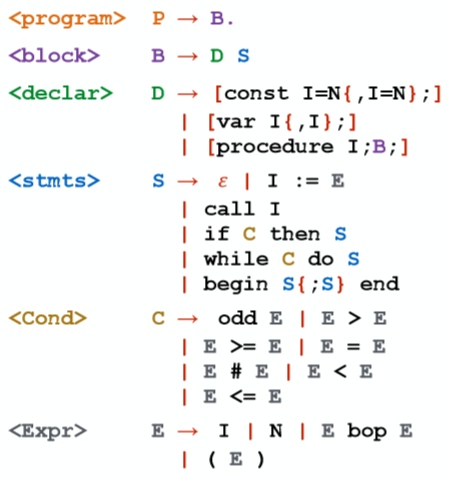
\includegraphics[width=\textwidth, height=\textheight, keepaspectratio]{pl01.png} 
		\caption{Sintassi di PL0}
	\end{subfigure}
	\hfill
	\begin{subfigure}{0.49\textwidth}
		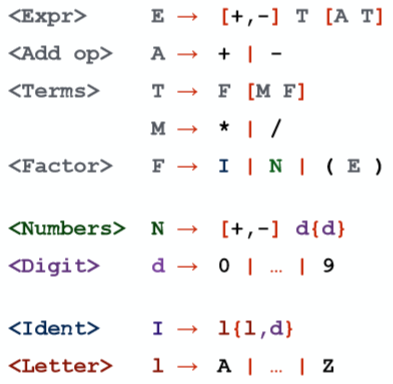
\includegraphics[width=\textwidth, height=\textheight, keepaspectratio]{pl02.png}
		\caption{Espressioni non ambigue e grammatica completa}
	\end{subfigure}
\end{figure}


% CAPITOLO 3
\chapter{Espressioni}
Abbiamo detto che le espressioni sono oggetti sintattici usati per ragionare sui loro significati, che sono i \textit{valori}. Per associare significati/valori alle espressioni, esse devono essere \textit{valutate}.

\section{Valori esprimibili}
Il valore ottenuto mediante la valutazione di una espressione è detto valore esprimibile. In generale, abbiamo espressioni che rappresentano \textit{interi} e \textit{booleani}.

\noindent
\begin{center}
	\begin{tabular}{lll}
	\toprule
	\textbf{NOME} & \textbf{DESCRIZIONE} & \textbf{METAVARIABILE} \\
	\midrule
	Valori esprimibili & $EVal = bool \cup int$ & $ev ::= k$ \\
	\bottomrule
\end{tabular}
\end{center}

\section{Espressioni aritmetiche}
Gli aspetti che le caratterizzano sono:
\begin{itemize}
	\item \textit{Regole di precedenza e associatività} per gli operatori.
	\item \textit{Ordine di valutazione} degli operandi.
	\item Presenza di \textit{side-effects} (qualunque effetto che non consiste puramente nella rappresentazione di valori).
	\item \textit{Overloading} degli operatori (simboli di operatore che hanno significato diverso a seconda del tipo degli operatori a cui sono applicati).
	\item \textit{Espressioni con tipi misti} (espressioni che combinano tipi diversi di valori).
	\item \textit{Arietà} dell'operatore (numero di operandi) e \textit{notazione}.
\end{itemize}

\section{Notazione}
La notazione specifica in che modo gli operandi e gli operatori vengono rappresentati, per indicare su quali operandi un operatore opera.
\newpage
\noindent
Abbiamo tre notazioni possibili:
\begin{itemize}
	\item Notazione \textit{in-fissa}: $a + b$.
	\item Notazione \textit{post-fissa}: $a b +$.
	\item Notazione \textit{pre-fissa}: $+ a b$.
\end{itemize}
La più usata nelle espressioni aritmetiche è quella in-fissa perché più facile ed intuitiva; però è anche quella in cui bisogna specificare altre regole (associatività, precedenza) o strumenti (parentesi) per eliminare l'\textit{ambiguità}. Nelle altre notazioni, infatti, l'arietà dell'operatore è spesso sufficiente ad evitare l'ambiguità.

\subsection{Notazione in-fissa}
Per la notazione in-fissa è necessario stabilire le regole di precedenza e associatività. Inoltre è necessario l'utilizzo delle parentesi. Le \textit{regole di precedenza} di un operatore definiscono l'ordine in cui vengono valutati gli operatori ``adiacenti'' a diversi livelli di precedenza. I \textit{livelli di precedenza} più tipici sono:
\begin{enumerate}
	\item Parentesi
	\item Operatori unari
	\item $**$
	\item $*,/$
	\item $+,-$
\end{enumerate}
Le \textit{regole di associatività} definiscono l'ordine con cui vengono valutati operatori allo stesso livello di precedenza. La regola di associatività più tipica è la valutazione \textit{da sinistra verso destra}.

\subsection{Notazione post-fissa}
La notazione post-fissa è più semplice di quella in-fissa, in quanto non necessita né di regole di precedenza e associatività né di parentesi. Serve però conoscere l'arietà degli operatori. La \textit{valutazione} evolve da sinistra a destra usando una pila LIFO.

\subsection{Notazione pre-fissa}
Anche la notazione pre-fissa è più semplice di quella in-fissa, in quanto non necessita né di regole di precedenza e associatività né di parentesi. Anche per essa serve però conoscere l'arietà degli operatori. La \textit{valutazione} evolve sempre da sinistra verso destra usando una pila LIFO, ma in questo caso ogni volta che viene letto un operatore devo contare gli operandi da leggere prima di eseguire il calcolo.
\begin{figure}[htp]
	\begin{subfigure}{0.49\textwidth}
		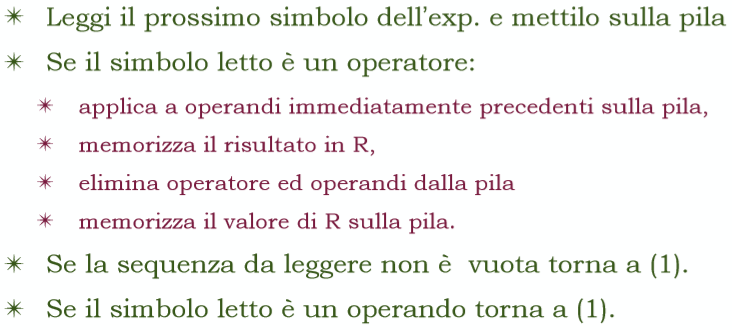
\includegraphics[width=\textwidth, height=\textheight, keepaspectratio]{post1.png} 
		\caption{Algoritmo di valutazione (post-fissa)}
	\end{subfigure}
	\rulesep
	\begin{subfigure}{0.49\textwidth}
		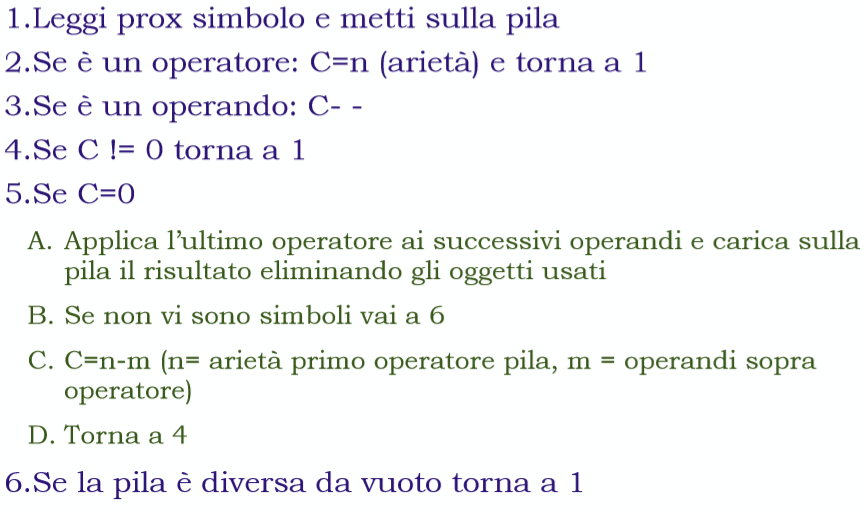
\includegraphics[width=\textwidth, height=\textheight, keepaspectratio]{pre1.png} 
		\caption{Algoritmo di valutazione (pre-fissa)}
	\end{subfigure}
	\begin{subfigure}{0.49\textwidth}
		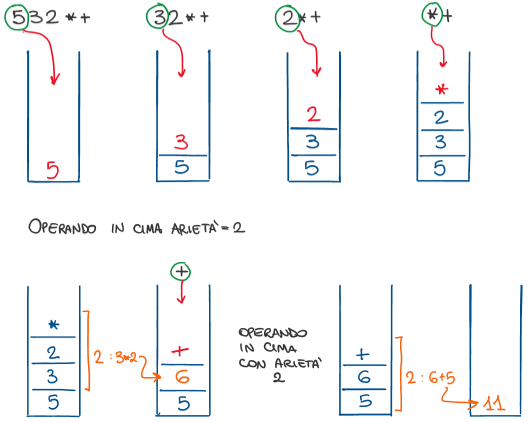
\includegraphics[width=\textwidth, height=\textheight, keepaspectratio]{post2.png}
		\caption{Esempio (post-fissa)}
	\end{subfigure}
	\rulesep
	\begin{subfigure}{0.49\textwidth}
		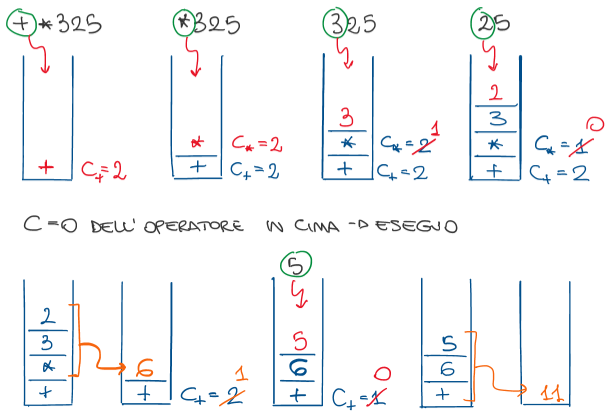
\includegraphics[width=\textwidth, height=\textheight, keepaspectratio]{pre2.png}
		\caption{Esempio (pre-fissa)}
	\end{subfigure}
\end{figure}

\section{Valutazione delle espressioni}
L'implementazione di un linguaggio di programmazione deve rappresentare internamente le espressioni, in modo da poterle manipolare.

Tipicamente, le espressioni sono rappresentate da \textit{alberi} che ne forniscono la struttura (con l'eliminazione di eventuali ambiguità legate a precedenze e associatività), ma che non possono dare informazioni riguardanti l'\textit{ordine di valutazione}.

Siccome ci sono vari aspetti che possono influire sul risultato delle espressioni, è importante sapere se un linguaggio usa una valutazione:
\begin{itemize}
	\item \textit{Lazy}, cioè valuta gli operandi solo quando necessario.
	\item \textit{Eager}, cioè se tutti gli operandi vengono comunque valutati. 
\end{itemize}
Gli aspetti citati in precedenza sono:
\begin{itemize}
\item \textit{Operandi non definiti} (divisione per 0).
\begin{lstlisting}
a == 0 ? b : b/a
\end{lstlisting}
\item \textit{Effetti collaterali} (quando una funzione cambia i propri parametri).
\begin{lstlisting}
fun(var) {
	var++;
}

a = 10;
b = a + fun(&a);
\end{lstlisting}
\item \textit{Aritmetica finita} (esiste un massimo numero rappresentabile).
\end{itemize}

\section{Semantica delle espressioni}
Dobbiamo dare significato alla seguente \textit{grammatica} delle espressioni:
\begin{figure}[htp]
	\centering
	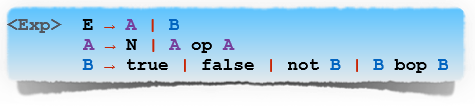
\includegraphics[width=0.7\textwidth]{exp.png}
\end{figure}
\\
Per prima cosa dobbiamo definire alcuni \textit{insiemi}:
\begin{itemize}
	\item Espressioni $\mathcal{E}$, insieme di espressioni valutate ad intero o booleano (alberi di valutazione) con metavariabile $e$
	\item Numeri $\mathcal{N}$, insieme di numeri della macchina sottostante con metavariabili $m, n, p$
	\item Booleani $\mathcal{B}$, insieme di valori booleani (true, false) con metavariabile $t$			
\end{itemize}
Ora usiamo questi insiemi per definire il \textit{sistema di transizione}, le cui regole forniranno esattamente la semantica operazionale delle espressioni di cui abbiamo dato la grammatica:
\[ \Gamma = \mathcal{E}, \text{ T} = \mathcal{N} \cup \mathcal{B}, \text{ op} \in \text{\{+,-,*,/\}, bop} \in \text{\{=,or\}} \]

\subsection{Regole}
\begin{figure}[htp]
	\centering
	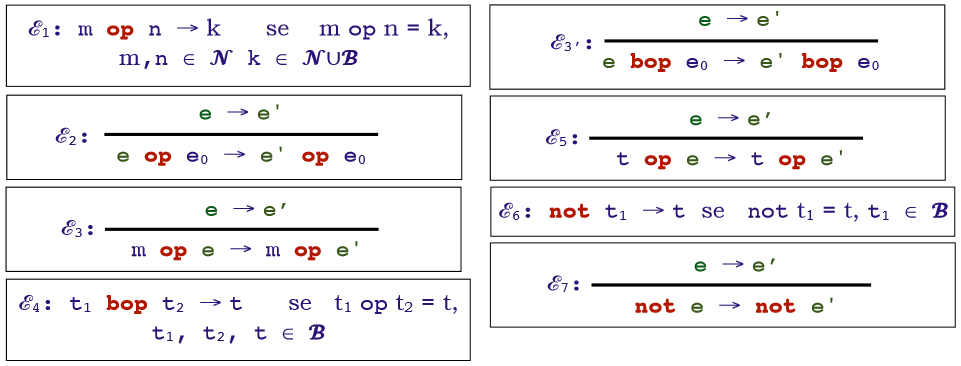
\includegraphics[width=\textwidth, height=\textheight, keepaspectratio]{expRegole1.png}
\end{figure}

\subsection{Valutazione ed equivalenza}
La funzione di \textit{valutazione} di espressioni $Eval: \mathcal{E} \rightarrow \mathcal{N} \cup \mathcal{B}$ che descrive il comportamento dinamico delle espressioni restituendo il valore in cui esse sono valutate, è definita come:
\[ Eval(e)=k \iff e \to^* k \]
La funzione di \textit{equivalenza} di espressioni $\equiv$ $\subseteq \mathcal{E} \times \mathcal{E}$ è definita come:
\[ e_0 \equiv e_1 \iff Eval(e_0)=Eval(e_1) \]


% CAPITOLO 4
\chapter{Ambienti}
Gli ambienti sono insiemi di legami (\textit{bindings}) associati agli \textit{identificatori}.

\section{Identificatori}
Gli identificatori sono sequenze di caratteri usate per rappresentare o denotare un altro oggetto. L'uso di nomi è fondamentale in quanto gli oggetti simbolici sono più facili da ricordare e permettono di attuare un processo di \textit{astrazione}. Inoltre, un identificatore può denotare più elementi, e un elemento può essere denotato da più identificatori diversi (\textit{aliasing}). Infine, gli identificatori non possono essere stringhe di caratteri qualunque, ma devono seguire delle regole in modo che il parser del linguaggio li possa riconoscere come tali.

\noindent
\begin{center}
	\begin{tabular}{lll}
		\toprule
		\textbf{NOME} & \textbf{DESCRIZIONE} & \textbf{METAVARIABILE} \\
		\midrule
		Identificatori & \lstinline|Id = {rate, a25, b, x, ...}| &  $ id, x $ \\
		\bottomrule
	\end{tabular}
\end{center}

\section{Bindings}
Il concetto di binding viene ereditato dalla matematica. Per prima cosa si ``dichiara'' il nome e il suo significato (\textit{binding occurrences}); successivamente il nome viene usato per rappresentare il suo significato (\textit{applied occurrences}); inoltre, un nome non dichiarato è un nome che può rappresentare qualunque cosa e quindi una sua occorrenza può essere legata a qualunque oggetto (\textit{free occurrences}). Infine, il raggio di azione di una definizione (\textit{scope}) definisce lo spazio in cui si può usare un nome per rappresentare il significato associato da un binding.
\newpage
\begin{figure}[htp]
	\begin{subfigure}{0.49\textwidth}
		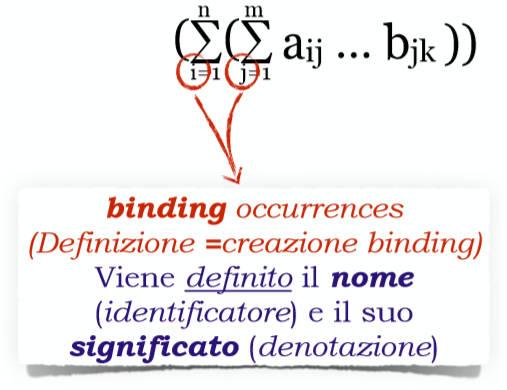
\includegraphics[width=\textwidth, height=\textheight, keepaspectratio]{bocc.png} 
		\caption{Binding occurrences}
	\end{subfigure}
	\begin{subfigure}{0.49\textwidth}
		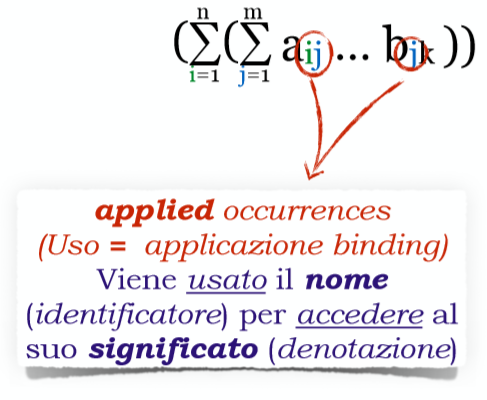
\includegraphics[width=\textwidth, height=\textheight, keepaspectratio]{aocc.png}
		\caption{Applied occurrences}
	\end{subfigure}
	\begin{subfigure}{0.49\textwidth}
		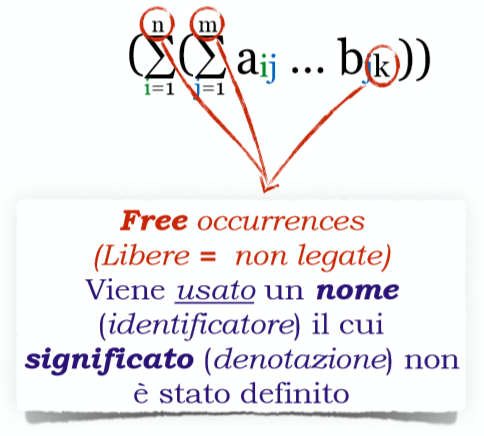
\includegraphics[width=\textwidth, height=\textheight, keepaspectratio]{focc.png} 
		\caption{Free occurrences}
	\end{subfigure}
	\begin{subfigure}{0.49\textwidth}
		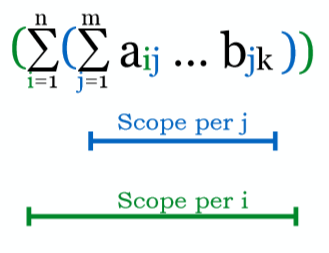
\includegraphics[width=\textwidth, height=\textheight, keepaspectratio]{scope.png}
		\caption{Scope di un binding}
	\end{subfigure}
\end{figure}

\subsection{Tipi di bindings}
Nei \textit{linguaggi di programmazione} i concetti di binding e scope prendono una connotazione propria:
\begin{itemize}
	\item Un identificatore è in posizione di \textit{definizione} (binding occurrence) quando si (ri)definisce il significato dell'identificatore.
	\item Un identificatore è in posizione di \textit{uso} (applied occurrence) quando si denota il significato definito da una definizione.
	\item Un identificatore è in posizione \textit{libera} (free occurrence) se il suo uso non è nel raggio di azione (scope) di una definizione.
\end{itemize}
I bindings possono legare nomi a diversi tipi di significato:
\begin{itemize}
	\item \textit{Nome-Valore}, quando il legame non può cambiare (costante).
	\item \textit{Nome-Locazione}, quando abbiamo una variabile (per non modificare il binding alla memoria).
	\item \textit{Locazione-Valore}, quando abbiamo una variabile (per modificare il valore del suo contenitore).
\end{itemize}
Esistono quindi i seguenti tipi di bindings:
\begin{itemize}
	\item \textit{Binding statico}, se occorre per la prima volta prima dell'esecuzione e rimane invariato durante tutta l'esecuzione del programma.
	\item \textit{Binding dinamico}, se occorre durante l'esecuzione e può variare.
\end{itemize}

\subsection{Tempi di bindings}
È importante anche stabilire quando avviene la creazione dei bindings, ovvero a tempo di compilazione (\textit{early binding}) o a tempo di esecuzione (\textit{late binding}). Nel primo caso abbiamo: allocazione statica della memoria, esecuzione veloce, programmazione poco flessibile. Nel secondo caso, invece, abbiamo: allocazione dinamica della memoria, esecuzione lenta, programmazione flessibile. Altri esempi di tempi di bindings sono:
\begin{itemize}
	\item Tempo di \textit{progettazione} (legami ai simboli).
	\item Tempo di \textit{implementazione} (legame del tipo floating point con la propria rappresentazione).
	\item Tempo di \textit{compilazione} (legami di tipo).
	\item Tempo di \textit{caricamento} (legami di variabili statiche alle celle di memoria).
	\item Tempo di \textit{esecuzione} (legami di variabili non statiche alle celle di memoria).
\end{itemize}

\section{Ambiente dinamico}
Ora possiamo dire che un \textit{ambiente} è l'insieme delle associazioni fra nomi e oggetti denotabili esistenti a run-time in uno specifico punto del programma ed in uno specifico momento dell'esecuzione.

La \textit{dichiarazione} quindi è un meccanismo (implicito o esplicito) col quale si crea un'associazione nell'ambiente; infatti, quando abbiamo delle occorrenze senza nessun legame in una espressione (free occurrences), vogliamo dar loro significato (per renderle applied occurrences), e con le dichiarazioni costruiamo le binding occurrences che rendono l'identificatore legato e non più libero.

L'\textit{ambiente dinamico} associa identificatori a valori denotabili ($\bot$ va associato all'identificatore che non è associato ad alcun valore). Un ambiente dinamico (con metavariabile $\rho$) è un elemento dello spazio di funzioni 
\[ Env=\bigcup\limits_{I \subseteq_f Id} Env_I \]
\begin{center}
	dove
\end{center}
\[ Env_I: I \rightarrow DVal \cup \{\bot\} \]

\newpage
\section{Semantica per espressioni con identificatori}
Dobbiamo dare significato alla seguente \textit{grammatica} delle espressioni (arricchita con gli identificatori):
\begin{figure}[htp]
	\centering
	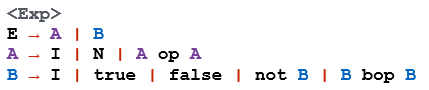
\includegraphics[width=0.7\textwidth]{expId.png}
\end{figure}
\\
Usando il nuovo insieme $\mathcal{E}^V$ delle espressioni (con identificatori) valutate ad intero o booleano (alberi di valutazione) con metavariabile $e$, definiamo il \textit{sistema di transizione} come:
\[ \Gamma = \mathcal{E}^V, \text{ T} = \mathcal{N} \cup \mathcal{B}, \text{ op} \in \text{\{+,-,*,/\}, bop} \in \text{\{=,or\}} \]

\subsection{Regole}
\begin{figure}[htp]
	\centering
	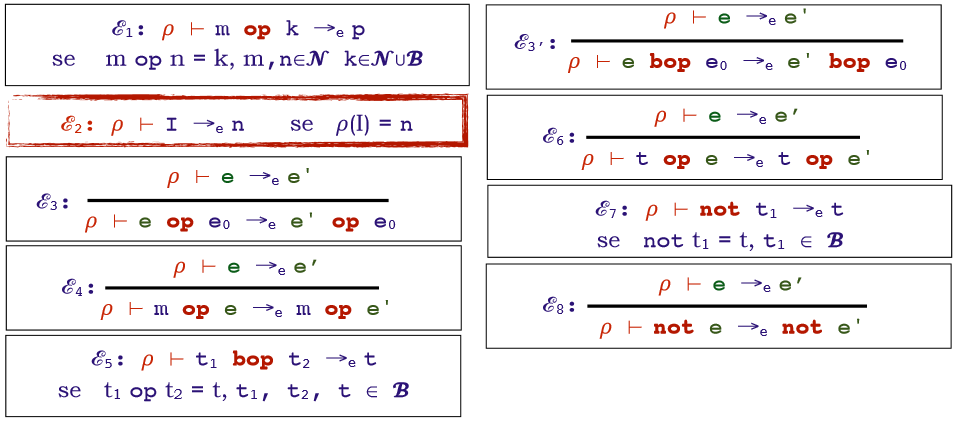
\includegraphics[width=\textwidth]{expRegole2.png}
\end{figure}

\subsection{Identificatori nelle espressioni}
La funzione $FI: Exp \rightarrow Id$ che ad ogni espressione associa l'insieme degli \textit{identificatori liberi} in essa contenuti, è definita per induzione da:
\[ FI(k) = \varnothing \]
\[ FI(id) = \{id\} \]
\[ FI(e_0 \text{ \lstinline|bop| } e_1) = FI(e_0) \cup FI(e_1) \]
\[ FI(\text{\lstinline|uop| } e) = FI(e) \]

\subsection{Termini chiusi e ground}
\begin{itemize}
	\item In un linguaggio (con identificatori), un termine in cui non ci sono identificatori liberi è detto \textit{termine chiuso}.
	\item In un linguaggio (con identificatori), un termine in cui non ci sono identificatori è detto \textit{termine ground}.
\end{itemize}

\section{Il tipo}
Il tipo determina il \textit{range di valori} che un identificatore può denotare e l'\textit{insieme di operazioni} definite su quei valori. I tipi sono utili, per motivi diversi, a vari livelli:
\begin{itemize}
	\item Livello di \textit{progetto}, perché organizzano l'informazione.
	\item Livello di \textit{programma}, perché identificano e prevengono errori.
	\item Livello di \textit{implementazione}, perché permettono alcune ottimizzazioni.
\end{itemize}

\subsection{Type binding}
Il \textit{tipo} può essere specificato in due modi:
\begin{itemize}
	\item Dichiarazione \textit{esplicita}, ovvero quando esiste un comando del linguaggio che permette di dichiarare il tipo delle variabili.
	\item Dichiarazione \textit{implicita}, ovvero quando esiste un meccanismo di default che specifica il tipo delle variabili attraverso convenzioni.
\end{itemize}
Anche il \textit{legame} che associa il tipo può avvenire in due modi:
\begin{itemize}
	\item \textit{Statico}, quando il tipo è associato a tempo di compilazione (rimane inalterato per l'intera esecuzione).
	\item \textit{Dinamico}, quando il tipo è associato con l'assegnamento (può cambiare durante l'esecuzione).
\end{itemize}

\section{Ambiente statico}
L'\textit{ambiente statico} associa agli identificatori il tipo degli oggetti che denoteranno ($\bot$ rappresenta il tipo di un identificatore non inizializzato). Un ambiente statico (con metavariabile $\Delta$) è un elemento dello spazio di funzioni	
\[ TEnv=\bigcup\limits_{I \subseteq_f Id} TEnv_I \]
\begin{center}
	dove
\end{center}
\[ TEnv_I: I \rightarrow DTyp \]

\subsection{Compatibilità di ambienti}
Sia $\rho:I$ un ambiente dinamico e $\Delta:I$ un ambiente statico con $I \subseteq_f Id$. Gli ambienti $\rho$ e $\Delta$ sono \textit{compatibili} (scritto $\rho:\Delta$) se e soltanto se 
\[ \forall id \in I. \left( \Delta(id)=\tau \wedge \rho(id) \in \tau \right) \]
Ovvero, un ambiente statico e uno dinamico sono compatibili se parlano in modo coerente degli stessi identificatori.

\section{Semantica statica delle espressioni}
Dobbiamo definire uno strumento formale che permetta la creazione di legami di tipo e la verifica della corretta forma delle espressioni. Questo strumento consiste nella cosiddetta \textit{semantica statica} che permette di associare un tipo ad ogni espressione corretta; in tal caso l'espressione è detta ben formata. A questo punto, la semantica per la valutazione delle espressioni diventa \textit{semantica dinamica}.

\subsection{Regole (semantica statica)}
\begin{figure}[htp]
	\centering
	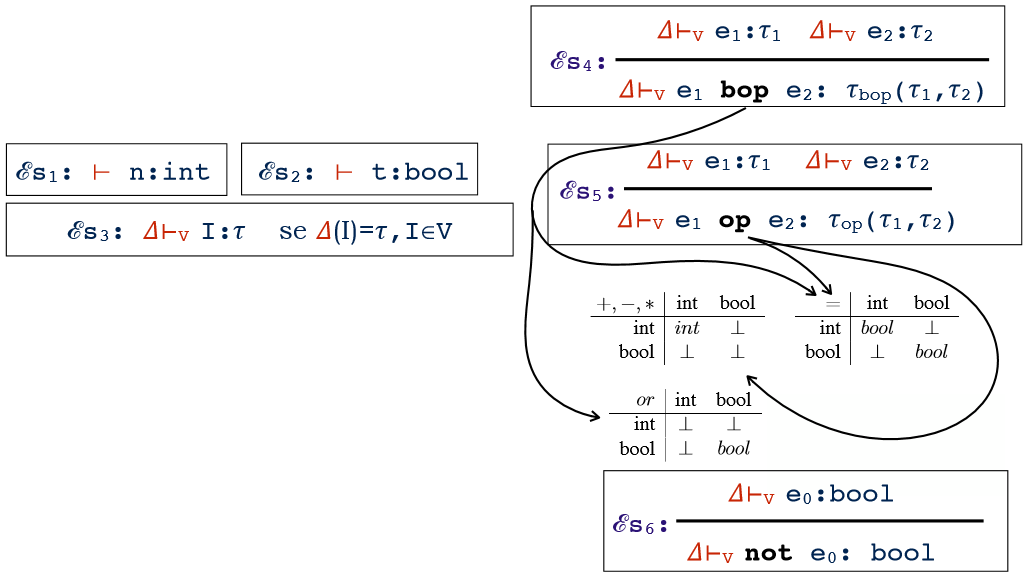
\includegraphics[width=0.9\textwidth]{expRegole3.png}
\end{figure}

\subsection{Regole (semantica dinamica)}
L'ultima modifica di forma delle regole per la valutazione delle espressioni riguarda il fatto che ora non guardiamo più all'ambiente dinamico specificando l'insieme degli identificatori, ma specificando l'ambiente statico compatibile.
\begin{figure}[htp]
	\centering
	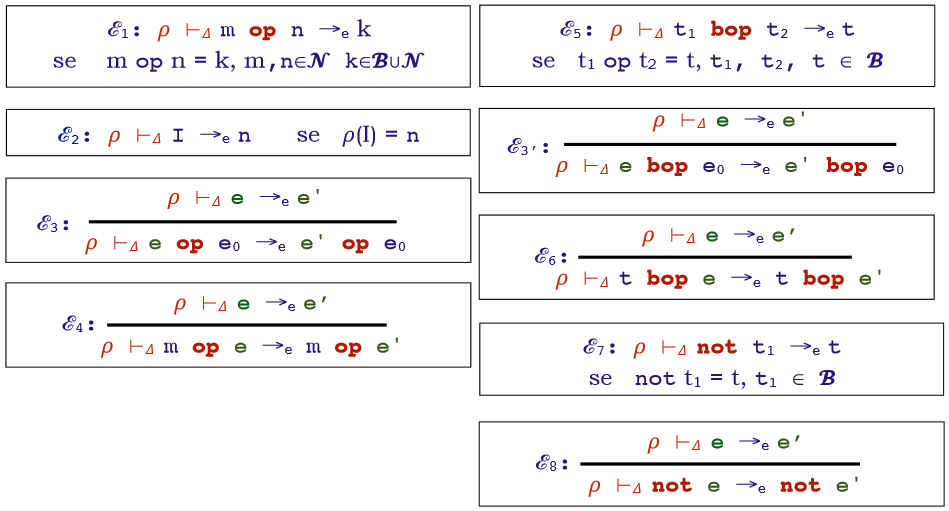
\includegraphics[width=0.9\textwidth]{expRegole4.png}
\end{figure}


% CAPITOLO 5
\chapter{Dichiarazioni}
Ricordiamo che le dichiarazioni denotano richieste di modifica/creazione di ambienti (legami tra identificatori e oggetti denotati); le dichiarazioni devono quindi essere elaborate per ottenere l'associazione che descrivono.

\section{Grammatica delle dichiarazioni}
Dobbiamo dare significato alla seguente \textit{grammatica} delle dichiarazioni:
\begin{figure}[htp]
	\centering
	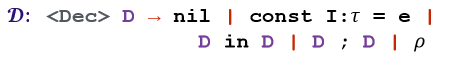
\includegraphics[width=0.7\textwidth]{dec.png}
\end{figure}
\\
Descriviamo ora le \textit{regole} una per una:
\begin{center}
	\begin{tabular}{lll}
		\toprule
		\textbf{REGOLA} & \textbf{DESCRIZIONE} & \textbf{SEMANTICA} \\
		
		\midrule
		\lstinline|nil| & Dichiarazione vuota & \hyperref[sec:decSemStat1]{$\mathcal{D}_{S_1}$} e \hyperref[sec:decSemDin1]{$\mathcal{D}_1$} \\
		
		\midrule
		\lstinline|const I:$\tau$=e| & Costante \textit{I} di tipo $\tau$ e valore \textit{e} & \hyperref[sec:decSemStat1]{$\mathcal{D}_{S_3}$} e \hyperref[sec:decSemDin1]{$\mathcal{D}_2$, $\mathcal{D}_3$} \\
		
		\midrule
		$\rho$ & Ambiente & \hyperref[sec:decSemStat1]{$\mathcal{D}_{S_2}$} \\
		
		\midrule
		$D_1 \text{\lstinline|;|} D_2$ & Composizione sequenziale & \hyperref[sec:decSemStat1]{$\mathcal{D}_{S_5}$} e \hyperref[sec:decSemDin1]{$\mathcal{D}_4$, $\mathcal{D}_5$, $\mathcal{D}_6$} \\
		
		\midrule
		$D_1 \text{ \lstinline|in| } D_2$ & Composizione privata & \hyperref[sec:decSemStat1]{$\mathcal{D}_{S_4}$} e \hyperref[sec:decSemDin1]{$\mathcal{D}_7$, $\mathcal{D}_8$, $\mathcal{D}_9$} \\
		
		\bottomrule
	\end{tabular}
\end{center}

\section{Dichiarazioni composte}
Nella \textit{composizione sequenziale} di dichiarazioni $D_1 \text{\lstinline|;|} D_2$, tutto ciò che è definito da $D_1$ è visibile da $D_2$ e anche all'esterno. Nella \textit{composizione privata} di dichiarazioni $D_1 \text{ \lstinline|in| } D_2$, invece, i legami creati da $D_1$ sono visibili e utilizzabili da $D_2$ ma non sono visibili all'esterno.
\begin{figure}[htp]
	\begin{subfigure}{0.49\textwidth}
		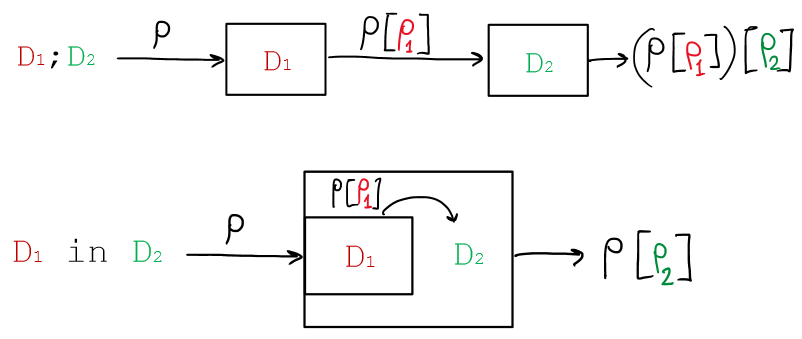
\includegraphics[width=\textwidth, height=\textheight, keepaspectratio]{decComp.png} 
		\caption{Visibilità degli ambienti}
	\end{subfigure}
	\hfill
	\begin{subfigure}{0.49\textwidth}
		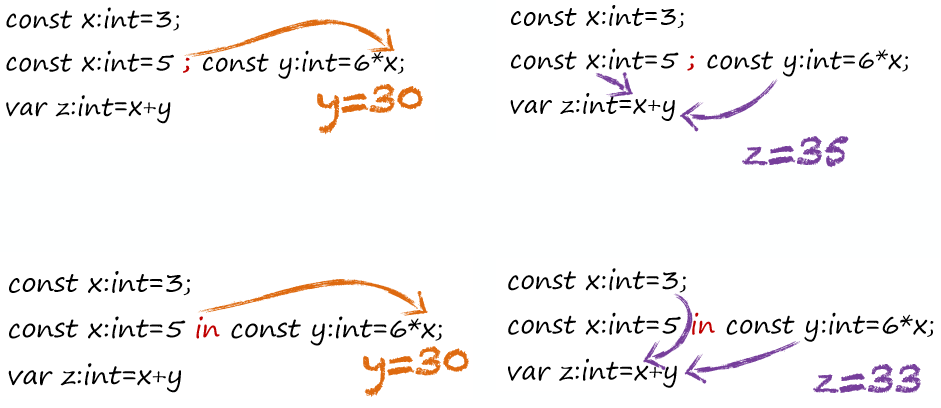
\includegraphics[width=\textwidth, height=\textheight, keepaspectratio]{decCompEs.png}
		\caption{Esempio}
	\end{subfigure}
\end{figure}

\section{Identificatori definiti}
La funzione $DI: Dic \rightarrow \rho(Id)$ che associa ad ogni dichiarazione l'insieme degli identificatori che definisce, è definita per induzione da:
\[ DI(\text{\lstinline|nil|}) = \varnothing \]
\[ DI(\text{\lstinline|const x:$\tau$=e|}) = \{x\} \]
\[ DI(d_1 \text{\lstinline|;|} d_2) = DI(d_1) \cup DI(d_2) \]
\[ DI(d_1 \text{ \lstinline|in| } d_2) = DI(d_2) \]
\[ DI(\rho) = I \text{ dove \textit{I} dominio di $\rho$} \]

\section{Identificatori liberi}
La funzione $FI: Dic \rightarrow \rho(Id)$ che associa ad ogni dichiarazione l'insieme dei suoi identificatori liberi, è definita per induzione da:
\[ FI(\text{\lstinline|nil|}) = \varnothing \]
\[ FI(\text{\lstinline|const x:$\tau$=e|}) = FI(e) \]
\[ FI(d_1 \text{\lstinline|;|} d_2) = FI(d_1) \cup (FI(d_2) \smallsetminus DI(d_1)) \]
\[ FI(d_1 \text{ \lstinline|in| } d_2) = FI(d_1) \cup (FI(d_2) \smallsetminus DI(d_1)) \]
\[ FI(\rho) = \varnothing \]

\section{Semantica delle dichiarazioni}
La \textit{semantica statica} per le dichiarazioni deve associare un ambiente statico ad ogni dichiarazione scritta correttamente (ben formata). La \textit{semantica dinamica}, invece, stabilisce come vengono elaborate le dichiarazioni.

\subsection{Aggiornamento degli ambienti}
Si considerino due ambienti $\beta,\beta' \in Env$ dove $\beta:V$, $\beta':V'$ con $V,V' \subseteq Id$, ovvero $\beta$ è definito sugli identificatori in $V$ e $\beta'$ è definito sugli identificatori in $V'$. L'\textit{aggiornamento dell'ambiente} $\beta$ mediante l'ambiente $\beta'$ è l'ambiente $\beta'' \in Env$, denotato con $\beta[\beta']$ e definito come
\[
\beta''(I) =
	\begin{cases}
	\beta'(I)& \hspace{1.0cm} \text{se } I \in V' \\
	\beta(I)& \hspace{1.0cm} \text{altrimenti}
	\end{cases}
\]

\subsection{Regole (semantica statica)}
\label{sec:decSemStat1}
\begin{figure}[htp]
	\centering
	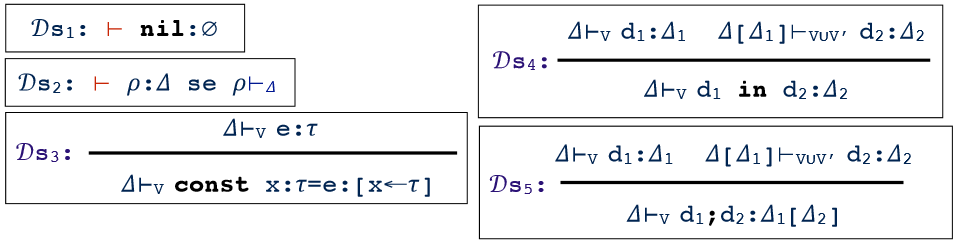
\includegraphics[width=\textwidth, height=\textheight, keepaspectratio]{decRegole1.png}
\end{figure}

\subsection{Regole (semantica dinamica)}
\label{sec:decSemDin1}
Usando l'insieme $\mathcal{D}$ delle dichiarazioni con identificatori elaborate in ambienti dinamici con metavariabile $d$, definiamo il \textit{sistema di transizione} come:
\[ \Gamma = \mathcal{D}, \text{ T} = Env \]
\begin{figure}[htp]
	\centering
	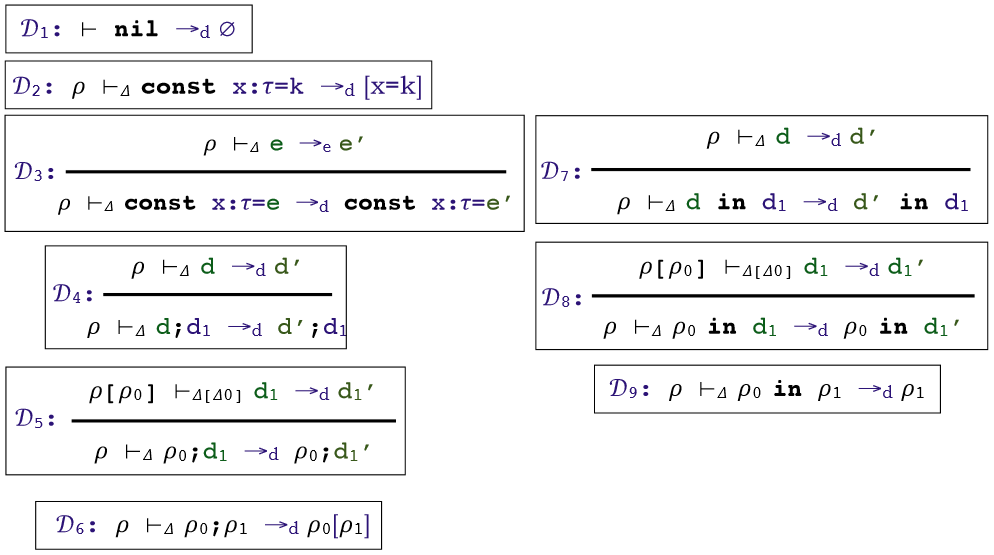
\includegraphics[width=\textwidth, height=\textheight, keepaspectratio]{decRegole2.png}
\end{figure}

\subsection{Elaborazione ed equivalenza}
La funzione di \textit{elaborazione} $Elab: \mathcal{D} \to Env$ che descrive il comportamento dinamico delle dichiarazioni restituendo l'ambiente in cui esse sono elaborate, è definita come:
\[ Elab(d)=\rho \iff d \rightarrow^* \rho \]
La funzione di \textit{equivalenza} di dichiarazioni $\equiv$ $\subseteq \mathcal{D} \times \mathcal{D}$ è definita come:
\[ d_0 \equiv d_1 \iff Elab(d_0)=Elab(d_1) \]


% CAPITOLO 6
\chapter{Memoria}
I comandi sono la categoria sintattica i cui elementi sono eseguiti per generare trasformazioni irreversibili di stato. In generale, l'astrazione dello stato della macchina è rappresentato dalla memoria. La \textit{memoria} non è altro che un insieme di associazioni tra locazioni e valori.

A questo punto, per poter trasformare lo stato, abbiamo bisogno di un meccanismo per trasformare memorie. Questo meccanismo è l'assegnamento, ovvero il comando che permette di modificare il contenuto della memoria. Siccome non è pensabile che chi programma possa utilizzare direttamente le locazioni di memoria, queste ultime vengono riferite attraverso identificatori che chiameremo variabili. Le \textit{variabili} quindi non sono altro che identificatori associati a locazioni, che a loro volta nella memoria sono associate a valori che possono cambiare durante l'esecuzione.
	
\section{Locazioni}
Per gestire tutta una serie di situazioni che coinvolgono identificatori variabili, abbiamo bisogno delle \textit{locazioni}. Alcuni esempi di queste situazioni sono:
\begin{itemize}
	\item Diversi oggetti chiamati con lo stesso nome (ridefinizione di variabili).
	\item Diversi nomi per lo stesso oggetto (aliasing).
	\item Nomi e valori di oggetti che cambiano nel tempo.
\end{itemize}
Abbiamo detto che lo stato della macchina viene rappresentato attraverso la sua memoria, ovvero attraverso l'insieme di associazioni tra locazioni (riferibili mediante variabili) e valori memorizzabili. La memoria, infatti, è lo strumento che utilizziamo nella nostra \textit{semantica} per tenere traccia dell'evoluzione dei valori delle variabili, attraverso la descrizione dei valori che stanno nelle locazioni associate alle variabili.

La locazione diventa quindi un valore denotabile, che modella l'indirizzo di memoria a cui la variabile è associata. Questo significa che la locazione viene creata da una \textit{dichiarazione} e avrà un tempo di vita determinato dallo scope (visibilità) della dichiarazione stessa.

\section{Variabili}
Le variabili, come le costanti, sono caratterizzate dai seguenti aspetti:
\begin{itemize}
	\item \textit{Nome/identificatore}, ovvero la sequenza di caratteri utilizzata per riferirsi all'oggetto denotato.
	\item \textit{Tipo}, ovvero l'insieme dei valori riferibili dall'oggetto e delle operazioni possibili su questi valori.
	\item \textit{Valore}, ovvero l'oggetto memorizzato nella locazione associata all'identificatore.
\end{itemize}
Gli aspetti propri delle sole variabili, invece, sono i seguenti:
\begin{itemize}
	\item \textit{Indirizzo/locazione}, ovvero l'astrazione della cella di memoria in cui il valore associato viene memorizzato.
	\item \textit{Scope}, ovvero il range dei comandi a cui la variabile è visibile.
	\item \textit{Tempo di vita}, ovvero tempo in cui il binding con la locazione è attivo.
\end{itemize}
Avendo introdotto un nuovo tipo di identificatore, ovvero la variabile, denotiamo con $\mathcal{D}^V$ il nuovo insieme delle \textit{dichiarazioni con variabili} e aggiungiamo che:
\[ DI(\text{\lstinline|var x:$\tau$=e|}) = \{x\} \]
\[ FI(\text{\lstinline|var x:$\tau$=e|}) = FI(e) \]
\begin{figure}[htp]
	\begin{subfigure}{0.49\textwidth}
		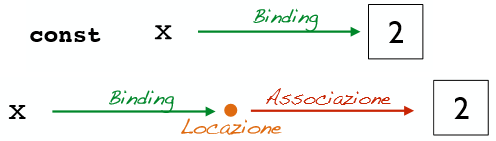
\includegraphics[width=\textwidth, height=\textheight, keepaspectratio]{constVar.png} 
		\caption{Costanti e variabili}
	\end{subfigure}
	\hfill
	\begin{subfigure}{0.49\textwidth}
		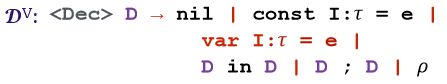
\includegraphics[width=\textwidth, height=\textheight, keepaspectratio]{decVar.png}
		\caption{Nuova grammatica per le dichiarazioni}
	\end{subfigure}
\end{figure}

\subsection{Regole (semantica statica)}
\label{sec:decSemStat2}
Aggiungiamo un nuovo tipo per permetterci di distinguere identificatori variabili e costanti. Definiamo quindi il tipo $\tau loc$ utilizzato per gli identificatori variabili di tipo $\tau$.
\begin{figure}[htp]
	\centering
	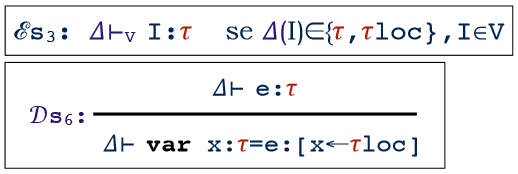
\includegraphics[width=0.9\textwidth]{varRegole.png}
\end{figure}

\section{Aggiornare la memoria}
Formalmente, una \textit{memoria} è un elemento dello spazio di funzioni $Mem$ definito da
\[ Mem=\bigcup\limits_{L \subseteq_f Loc} Mem_L \]
dove $Mem_L: L \rightarrow MVal$ ha metavariabile $\sigma$ e $MVal=\mathcal{N} \cup \mathcal{B}$ sono i valori memorizzabili.

Quindi, le \textit{locazioni} sono modellate come un insieme finito ma illimitato di elementi che rappresentano celle di memoria. Per garantire questo esiste la funzione $New(L) \in (Loc \smallsetminus L)$ che preso un insieme di locazioni già utilizzate, ne genera una nuova da utilizzare.

Si considerino ora due memorie $\sigma,\sigma' \in Mem$ dove $\sigma:L$, $\sigma':L'$ con $L,L' \subseteq Loc$, ovvero $\sigma$ è definito sulle locazioni in $L$ e $\sigma'$ è definito sulle locazioni in $L'$. L'\textit{aggiornamento della memoria} $\sigma$ mediante la memoria $\sigma'$ è la memoria $\sigma'' \in Mem$, denotato con $\sigma[\sigma']$ e definito come
\[
\sigma''(l) =
	\begin{cases}
	\sigma'(l)& \hspace{1.0cm} \text{se } l \in L' \\
	\sigma(l)& \hspace{1.0cm} \text{altrimenti}
	\end{cases}
\]

\section{Semantica con memoria}
Introdurre le variabili significa poter scrivere espressioni e dichiarazioni che contengono identificatori variabili. Questo implica che per valutare queste espressioni ed elaborare queste dichiarazioni abbiamo bisogno di integrare nel sistema di transizione anche la memoria da usare per valutare gli identificatori variabili. Quindi, il \textit{sistema di transizione delle espressioni} diventa:
\[ \Gamma^V = \mathcal{E}^V \times Mem, \text{ T}^V = (\mathcal{N} \cup \mathcal{B}) \times Mem \]
Mentre il \textit{sistema di transizione delle dichiarazioni} diventa:
\[ \Gamma^V = \mathcal{D}^V \times Mem, \text{ T}^V = Env \times Mem \]
Osserviamo che nelle espressioni la memoria non può essere trasformata dalla valutazione, che accede in memoria sempre e solo in lettura. Nelle dichiarazioni, invece, la memoria può essere diversa dopo la transizione, questo perché inizializzando le variabili si modifica la memoria.

\subsection{Valutazione ed equivalenza (con variabili)}
La funzione di \textit{valutazione} di espressioni $Eval: \mathcal{E}^V \times Mem \rightarrow (\mathcal{N} \cup \mathcal{B}) \times Mem$ che descrive il comportamento dinamico delle espressioni restituendo il valore in cui esse sono valutate (insieme alla \textit{memoria}), è definita come:
\[ Eval(\langle e,\sigma \rangle) = \langle k,\sigma \rangle \iff \langle e,\sigma \rangle \to^* \langle k,\sigma \rangle \]
La funzione di \textit{equivalenza} di espressioni con variabili $\equiv$ $\subseteq \mathcal{E}^V \times \mathcal{E}^V$ è definita come:
\[ e_0 \equiv e_1 \iff \forall \sigma.(Eval(\langle e_0,\sigma \rangle) = Eval(\langle e_1,\sigma \rangle)) \]

\subsection{Elaborazione ed equivalenza (con variabili)}
La funzione di \textit{elaborazione} $Elab: \mathcal{D}^V \times Mem \to Env \times Mem$ che descrive il comportamento dinamico delle dichiarazioni restituendo l'ambiente in cui esse sono elaborate, è definita come:
\[ Elab(\langle d,\sigma \rangle)=\rho \iff \langle d,\sigma \rangle \rightarrow^* \langle \rho,\sigma' \rangle \]
La funzione di \textit{equivalenza} di dichiarazioni con variabili $\equiv$ $\subseteq \mathcal{D}^V \times \mathcal{D}^V$ è definita come:
\[ d_0 \equiv d_1 \iff \forall \sigma.(Elab(\langle d_0,\sigma \rangle) = Elab(\langle d_1,\sigma \rangle)) \]

\subsection{Regole (espressioni con variabili)}
\begin{figure}[htp]
	\centering
	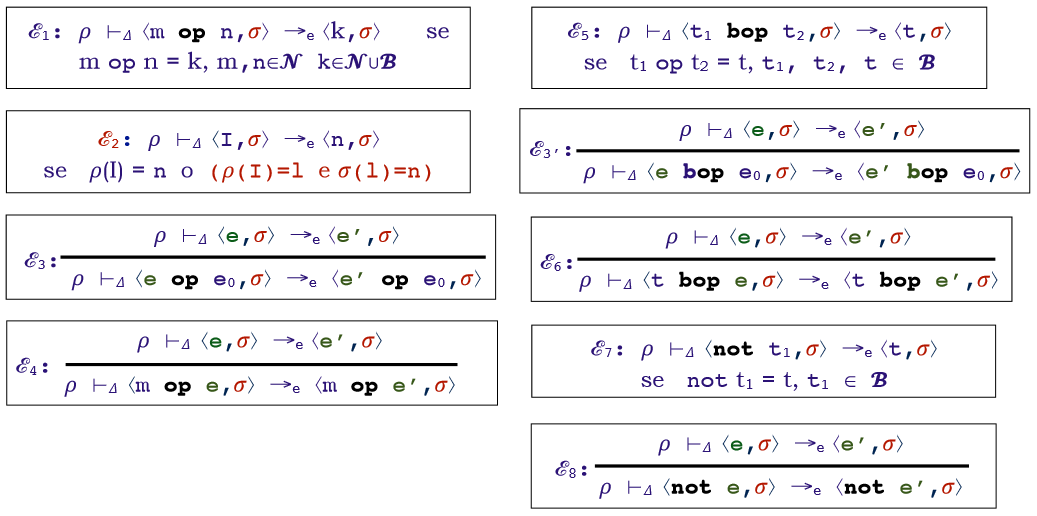
\includegraphics[width=\textwidth, height=\textheight, keepaspectratio]{expRegole5.png}
\end{figure}

\subsection{Regole (dichiarazioni con variabili)}
\label{sec:decSemDin2}
\begin{figure}[htp]
	\centering
	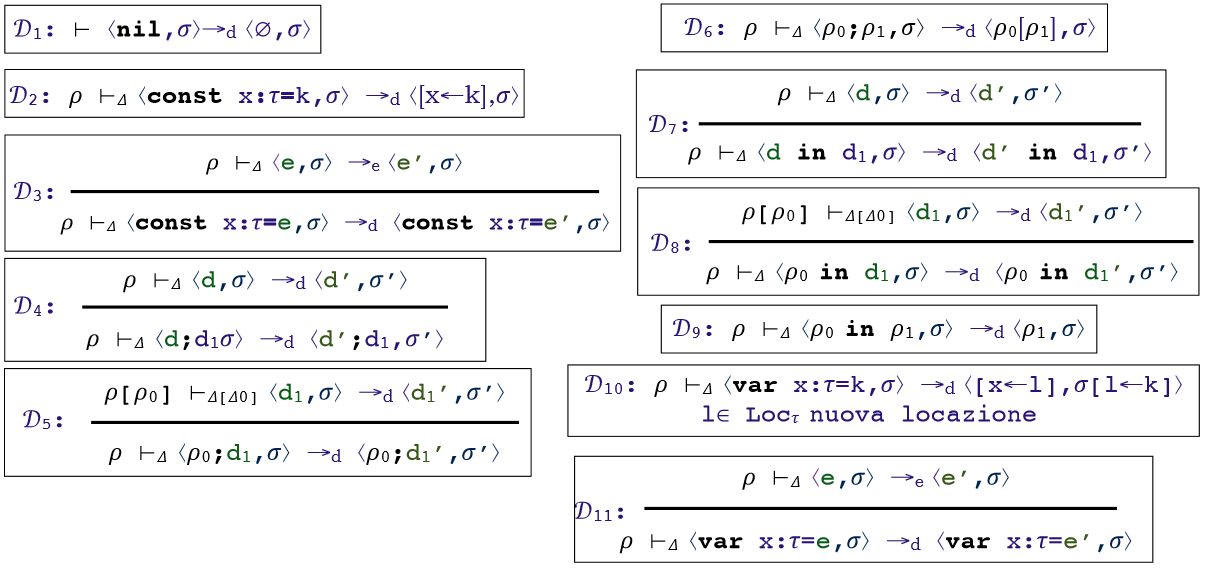
\includegraphics[width=\textwidth, height=\textheight, keepaspectratio]{decRegole3.png}
\end{figure}


% CAPITOLO 7
\chapter{Comandi}
Ricordiamo che il significato di un comando è essenzialmente quello di una trasformazione di stato (ovvero di memorie); i comandi devono quindi essere eseguiti per ottenere la richiesta di trasformazione della memoria.

\section{Grammatica dei comandi}
Dobbiamo dare significato alla seguente \textit{grammatica} dei comandi:
\begin{figure}[htp]
	\centering
	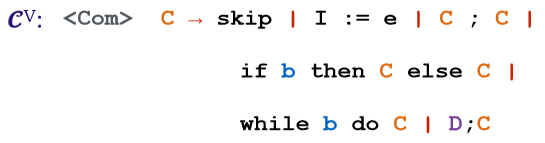
\includegraphics[width=0.7\textwidth]{com.png}
\end{figure}
\\
Descriviamo ora le \textit{regole} una per una:
\begin{center}
	\begin{tabular}{lll}
		\toprule
		\textbf{REGOLA} & \textbf{DESCRIZIONE} & \textbf{SEMANTICA} \\
		
		\midrule
		\lstinline|skip| & Comando nullo & \hyperref[sec:comSemStat]{$\mathcal{C}_{S_4}$} e \hyperref[sec:comSemDin]{$\mathcal{C}_8$} \\
		
		\midrule
		\lstinline|I := e| & Assegnamento & \hyperref[sec:comSemStat]{$\mathcal{C}_{S_1}$} e \hyperref[sec:comSemDin]{$\mathcal{C}_1$, $\mathcal{C}_2$} \\
		
		\midrule
		\lstinline|C ; C| & Composizione sequenziale & \hyperref[sec:comSemStat]{$\mathcal{C}_{S_3}$} e \hyperref[sec:comSemDin]{$\mathcal{C}_9$, $\mathcal{C}_{10}$} \\
		
		\midrule
		\lstinline|if b then C else C| & Comando condizionale & \hyperref[sec:comSemStat]{$\mathcal{C}_{S_2}$} e \hyperref[sec:comSemDin]{$\mathcal{C}_3$, $\mathcal{C}_4$, $\mathcal{C}_5$} \\
		
		\midrule
		\lstinline|while b do C| & Comando iterativo & \hyperref[sec:comSemStat]{$\mathcal{C}_{S_5}$} e \hyperref[sec:comSemDin]{$\mathcal{C}_6$, $\mathcal{C}_7$} \\
		
		\midrule
		\lstinline|D ; C| & Blocco & \hyperref[sec:comSemStat]{$\mathcal{C}_{S_6}$} e \hyperref[sec:comSemDin]{$\mathcal{C}_{11}$, $\mathcal{C}_{12}$, $\mathcal{C}_{13}$} \\
	
		\bottomrule
	\end{tabular}
\end{center}

\section{Assegnamento}
L'\textit{assegnamento} è il comando base che assegna il valore di una espressione ad un identificatore, chiamato anche variabile. Le \textit{variabili}, infatti, sono contenitori di valori con un nome particolare, il cui contenuto può essere modificato tramite un assegnamento. L'assegnamento, quindi, è costruito utilizzando un termine che denota la locazione da modificare (left-value) e un termine che contiene il nuovo valore da associare alla locazione (right-value).

\section{Comandi iterativi}
I comandi possono essere \textit{composti} sequenzialmente. In quel caso si avrà che tutte le trasformazioni eseguite dal primo comando sono il punto di partenza per le trasformazioni che deve eseguire il secondo. Inoltre, esiste anche il \textit{comando condizionale}, che sceglie tra l'esecuzione di due possibili comandi in funzione del valore (booleano) di una espressione detta guardia. Tuttavia, se vogliamo ripetere l'esecuzione di un comando (o di un comando composto) finché il valore di una espressione booleana rimane vero, abbiamo bisogno dell'\textit{iterazione} che, insieme alla ricorsione, permette di ottenere formalismi di calcolo Turing completi. L'iterazione può essere di due tipologie:
\begin{itemize}
	\item \textit{Indeterminata}, quando i cicli sono controllati logicamente su una espressione booleana (es. while).
	\item \textit{Determinata}, quando i cicli sono controllati numericamente con un numero di ripetizioni determinate all'inizio del ciclo (es. for).
\end{itemize}

\section{Blocchi}
Il \textit{blocco} serve per creare un ambiente locale al comando. Infatti, per eseguire un comando che coinvolge variabili abbiamo bisogno di combinare \textit{ambienti} (creati e aggiornati dalle dichiarazioni con modifiche reversibili) e \textit{memorie} (aggiornate mediante comandi con modifiche irreversibili). Il blocco, quindi, è il costrutto che ci permette di identificare l'ambiente in cui un comando viene eseguito e, in particolare, è una regione testuale che può contenere dichiarazioni locali e comandi. L'uso dei blocchi permette di:
\begin{itemize}
	\item Gestire localmente i nomi.
	\item Aumentare la chiarezza.
	\item Usare i nomi indipendentemente gli uni dagli altri.
	\item Eseguire comandi in ambienti modificati.
\end{itemize}

\subsection{Scope}
Solitamente, i blocchi sono identificati da delimitatori che ne determinano lo scope. Inoltre, i blocchi non possono essere parzialmente sovrapposti, ovvero o sono disgiunti o sono annidati. È quindi importante stabilire la seguente \textit{regola di visibilità} (scope) delle dichiarazioni: una dichiarazione locale ad un blocco è visibile in quel blocco e in tutti i blocchi in esso annidati, a meno che non intervenga in tali blocchi una nuova dichiarazione dello stesso nome (che nasconde la precedente).
\begin{figure}[htp]
	\begin{subfigure}{0.49\textwidth}
		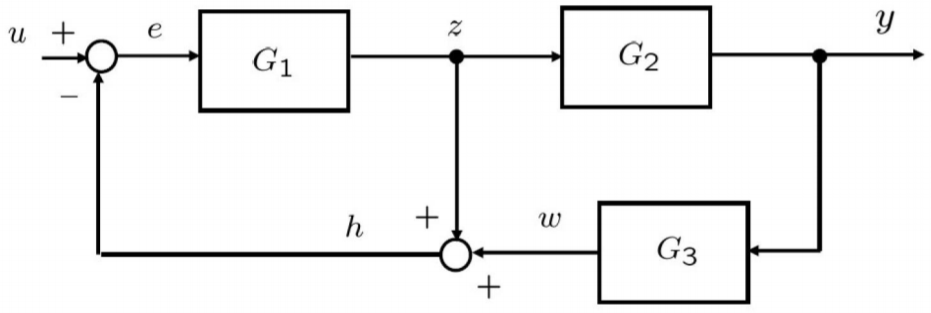
\includegraphics[width=\textwidth, height=\textheight, keepaspectratio]{blocchi1.png} 
		\caption{Blocchi annidati}
	\end{subfigure}
	\hfill
	\begin{subfigure}{0.49\textwidth}
		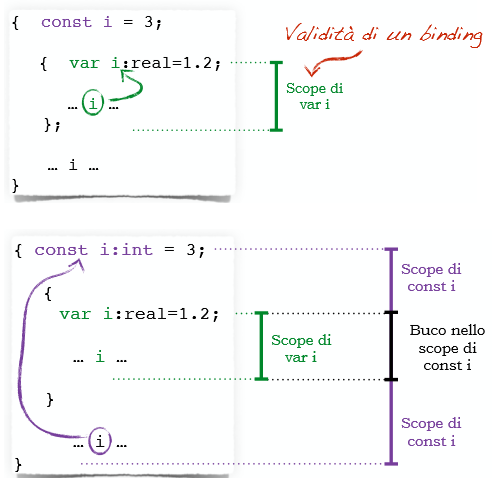
\includegraphics[width=\textwidth, height=\textheight, keepaspectratio]{blocchi2.png}
		\caption{Validità dei bindings nei blocchi}
	\end{subfigure}
\end{figure}
\newpage
\noindent
Come si vede dalla \textit{figura (b)}, ogni definizione annidata genera un buco nello scope precedente, ovvero nella porzione di codice in cui il binding è valido e il nome è utilizzabile con il significato associato.

Possiamo ora definire lo \textit{scope statico}, che si riferisce all'area del testo del programma nella quale tutte le occorrenze applicate (di uso) di un identificatore si riferiscono alla stessa occorrenza di binding dell'identificatore.

\subsection{Tipi di ambienti}
Lo scope di una variabile è quindi il range di comandi ai quali è visibile. Esistono quindi variabili di tipo diverso rispetto alla regione in cui sono definite:
\begin{itemize}
	\item Le \textit{variabili locali} di un blocco sono quelle dichiarate nel blocco stesso.
	\item Le \textit{variabili non locali} ad un blocco sono quelle visibili al blocco ma non dichiarate in esso.
	\item Le \textit{variabili globali} sono quelle dichiarate nel blocco che contiene l'intero programma.
\end{itemize}
Tali tipologie di variabili determinano la caratterizzazione di diversi tipi di ambienti:
\begin{itemize}
	\item \textit{Ambiente locale}, che contiene le associazioni create all'ingresso del blocco (variabili locali).
	\item \textit{Ambiente non locale}, che contiene le associazioni ereditate da altri blocchi ma visibili al blocco stesso.
	\item \textit{Ambiente globale}, che contiene quella parte di ambiente non locale relativo alle associazioni comuni a tutti i blocchi.
\end{itemize}

\newpage
\subsection{Tempo di vita}
Alla luce di quanto visto per ambienti e visibilità, dovrebbe essere chiaro che non sempre le variabili esistono per tutta la durata di un programma. Esse, infatti, hanno un \textit{tempo di vita}, ovvero il tempo di esecuzione nel quale tutte le occorrenze applicate di un identificatore si riferiscono alla stessa locazione di memoria. Il tempo di vita di una variabile inizia quando viene legata ad una specifica cella (allocazione) e termina quando il legame viene sciolto (deallocazione). Osserviamo quindi che scope e tempo di vita sono concetti molto vicini, ma di natura diversa. Infatti, lo scope è un concetto spaziale (definito a tempo di compilazione) mentre il tempo di vita è un concetto temporale (definito a tempo di esecuzione).
\begin{figure}[htp]
	\begin{subfigure}{0.49\textwidth}
		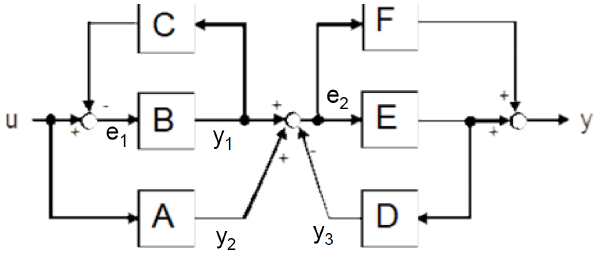
\includegraphics[width=\textwidth, height=\textheight, keepaspectratio]{blocchi3.png} 
		\caption{Tipi di ambienti}
	\end{subfigure}
	\hfill
	\begin{subfigure}{0.49\textwidth}
		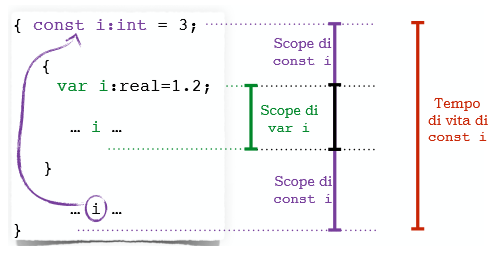
\includegraphics[width=\textwidth, height=\textheight, keepaspectratio]{blocchi4.png}
		\caption{Tempo di vita nei blocchi}
	\end{subfigure}
\end{figure}

\section{Identificatori liberi}
\[ FI(\text{\lstinline|x := e|}) = FI(e) \cup \{x\} \]
\[ FI(\text{\lstinline|if| }e\text{ \lstinline|then| }c_0\text{ \lstinline|else| }c_1) = FI(c_0) \cup FI(c_1) \cup FI(e) \]
\[ FI(c_0 \text{\lstinline|;|} c_1) = FI(c_0) \cup FI(c_1) \]
\[ FI(\text{\lstinline|while| }e\text{ \lstinline|do| }c) = FI(c) \cup FI(e) \]
\[ FI(d \text{\lstinline|;|} c) = FI(d) \cup (FI(c) \smallsetminus DI(d)) \]

\section{Identificatori definiti}
\[ DI(\text{\lstinline|x := e|}) = \varnothing \]
\[ DI(\text{\lstinline|if| }e\text{ \lstinline|then| }c_0\text{ \lstinline|else| }c_1) = DI(c_0) \cup DI(c_1) \]
\[ DI(c_0 \text{\lstinline|;|} c_1) = DI(c_0) \cup DI(c_1) \]
\[ DI(\text{\lstinline|while| }e\text{ \lstinline|do| }c) = DI(c) \]
\[ DI(d \text{\lstinline|;|} c) = DI(c) \cup DI(d) \]

\section{Semantica dei comandi}
La \textit{semantica statica} per i comandi serve solo a verificare che il comando sia ben formato, che rispetti cioè tutti i vincoli semantici. La \textit{semantica dinamica}, invece, stabilisce come vengono eseguiti i comandi. Definiamo quindi il seguente \textit{sistema di transizione}:
\[ \Gamma^V = \mathcal{C}^V \times Mem \cup Mem, \text{ T}^V = Mem \]

\subsection{Regole (semantica statica)}
\label{sec:comSemStat}
\begin{figure}[htp]
	\centering
	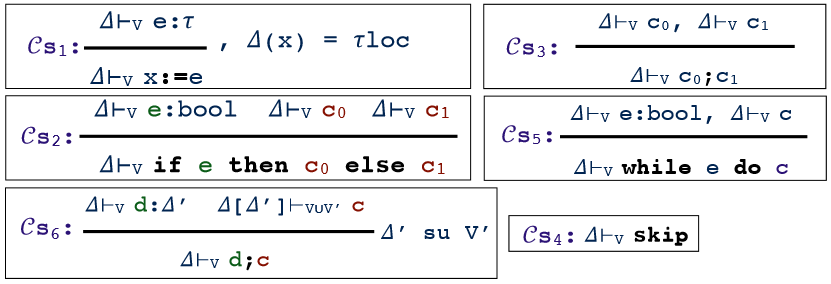
\includegraphics[width=\textwidth, height=\textheight, keepaspectratio]{comRegole1.png}
\end{figure}

\subsection{Regole (semantica dinamica)}
\label{sec:comSemDin}
\begin{figure}[htp]
	\centering
	\includegraphics[width=\textwidth, height=\textheight, keepaspectratio]{comRegole2.png}
\end{figure}

\subsection{Esecuzione ed equivalenza}
La funzione di \textit{esecuzione} $Exec: \mathcal{C}^V \times Mem \to Mem$ che descrive il comportamento dinamico dei comandi restituendo la memoria risultante dalle trasformazioni effettuate dai comandi eseguiti, è definita come:
\[ Exec(\langle c,\sigma \rangle)=\sigma' \iff \langle c,\sigma \rangle \rightarrow^* \sigma' \]
La funzione di \textit{equivalenza} di comandi $\equiv$ $\subseteq \mathcal{C}^V \times \mathcal{C}^V$ è definita come:
\[ c_0 \equiv c_1 \iff \forall \sigma.(Exec(\langle c_0,\sigma \rangle) = Exec(\langle c_1,\sigma \rangle)) \]


% CAPITOLO 8
\chapter{Procedure}
L'uso delle \textit{procedure} permette la cosiddetta astrazione del controllo. L'astrazione chiede di identificare le proprietà importanti di ciò che si vuole descrivere al fine di concentrarsi sulle questioni rilevanti ed ignorare le altre.

\section{Astrazione del controllo}
Le procedure sono lo strumento sintattico per l'\textit{astrazione del controllo}. Tale forma di astrazione è quella che ci interessa, in quanto il nostro obiettivo è quello di abbreviare la scrittura di programmi che contengono sequenze ripetute di comandi uguali che possono differire nei dati su cui operano. Ciò che viene fatto nel processo di astrazione del controllo consiste essenzialmente nel legare una sequenza di comandi (detta \textit{corpo} della procedura) ad un identificatore (detto \textit{nome} della procedura). Mantenendo solo nome e corpo potremmo però associare solo esecuzioni che fanno sempre la stessa cosa ogni volta che vengono richiamate. Per rendere l'esecuzione dipendente da altri elementi validi al momento della chiamata, abbiamo bisogno di un'altro aspetto da considerare, ovvero i \textit{parametri}. Nome e parametri formano quindi l'\textit{interfaccia}. Il corpo, invece, è ciò che viene valutato/elaborato/eseguito ogni qualvolta il nome è richiamato, con appropriati parametri, in qualche punto di programma.

\section{Sottoprogramma}
Quando si parla di astrazione del controllo nei linguaggi di programmazione, ci sono in realtà due categorie di sottoprogrammi che possiamo definire:
\begin{itemize}
	\item Le \textit{procedure}, ovvero collezioni di comandi che definiscono una computazione parametrizzata senza necessariamente restituire un risultato, ma solo una modifica di stato.
	\item Le \textit{funzioni}, che restituiscono un valore dopo aver eseguito modifiche di stato.
\end{itemize}
Un \textit{sottoprogramma} è quindi una porzione di codice identificato da un nome, dotato di un ambiente locale proprio e capace di scambiare informazioni con il resto del codice mediante fissati canali (parametri e/o valori di ritorno).
\\
Per caratterizzare un sottoprogramma dobbiamo specificarlo e scriverlo (tramite la \textit{definizione}) e poi dobbiamo poterlo usare (tramite la \textit{chiamata}).
\begin{figure}[htp]
	\centering
	\includegraphics[width=\textwidth, height=\textheight, keepaspectratio]{sottoprogramma.png}
\end{figure}

\section{Ambiente di riferimento}
Il concetto di visibilità (scope) può essere esteso in presenza di procedure. Ciò ci permette di definire il concetto di \textit{ambiente di riferimento} per un comando, ovvero la collezione di tutti i nomi che sono visibili al comando. L'ambiente di riferimento di una procedura è determinato da varie tipologie di regole:
\begin{itemize}
	\item \textit{Regole di scope} (statico o dinamico), che servono quando la procedura contiene un ambiente non locale.
	\item \textit{Regole specifiche} del linguaggio.
	\item \textit{Regole per il passaggio dei parametri}.
	\item \textit{Regole di binding} (shallow o deep), che intervengono quando una procedura è passata come parametro ad un'altra procedura.
\end{itemize}

\subsection{Tipi di scope}
In un linguaggio con \textit{scope statico}, l'ambiente di riferimento è costituito dalle variabili locali più tutte le variabili negli scope più esterni. In un linguaggio con \textit{scope dinamico}, l'ambiente di riferimento è l'insieme delle variabili locali più tutte le variabili visibili nei sottoprogrammi attivi (cioè quelli la cui esecuzione è iniziata e non è ancora terminata).

Nello \textit{scoping statico} (a tempo di compilazione), un nome non locale è risolto nel blocco che testualmente lo racchiude. Nello \textit{scoping dinamico} (a tempo di esecuzione), invece, un nome non locale è risolto nella chiamata attivata più di recente e non ancora terminata.
\begin{figure}[htp]
	\begin{subfigure}{0.49\textwidth}
		\includegraphics[width=\textwidth, height=\textheight, keepaspectratio]{scopeStatico.png} 
		\caption{Scoping statico}
	\end{subfigure}
	\hfill
	\begin{subfigure}{0.49\textwidth}
		\includegraphics[width=\textwidth, height=\textheight, keepaspectratio]{scopeDinamico.png}
		\caption{Scoping dinamico}
	\end{subfigure}
\end{figure}
\newpage
\noindent
Con scoping statico, si risale la catena di annidamento dei blocchi seguendo quella che viene chiamata \textit{catena statica} (nota a tempo di compilazione). Mentre con scoping dinamico, si risale la catena di chiamate dei blocchi seguendo quella che viene chiamata \textit{catena dinamica} (nota a tempo di esecuzione).
\begin{figure}[htp]
	\begin{subfigure}{0.49\textwidth}
		\includegraphics[width=\textwidth, height=\textheight, keepaspectratio]{catenaStatica.png} 
		\caption{Catena statica}
	\end{subfigure}
	\hfill
	\begin{subfigure}{0.49\textwidth}
		\includegraphics[width=\textwidth, height=\textheight, keepaspectratio]{catenaDinamica.png}
		\caption{Catena dinamica}
	\end{subfigure}
\end{figure}
\\
In definitiva, lo scope statico è più complesso da implementare (lento nella costruzione della catena), ma è più efficiente (veloce nei riferimenti). Lo scope dinamico, invece, è più semplice da implementare (veloce nella costruzione della catena), ma è meno efficiente (lento nei riferimenti) perché non sfrutta le informazioni date dal compilatore.

\section{Allocazione della memoria}
Risolvere un riferimento vuol dire tradurre/sostituire il nome con l'oggetto a cui si riferisce attraverso la risoluzione del suo legame/binding. L'identificazione del legame corretto dipende dal tipo di \textit{scope}: nel caso \textit{statico}, dobbiamo mantenere la catena statica (tempo di compilazione) che ci permette di riferire gli oggetti mediante indirizzi relativi ad un base address (indirizzo dell'RdA allocato a tempo di esecuzione) e ad un offset (dentro l'RdA); nel caso \textit{dinamico}, invece, basta seguire la catena dinamica (tempo di esecuzione) e cercare il riferimento in ogni RdA. Un concetto fortemente legato all'uso delle procedure è l'\textit{allocazione della memoria}, ovvero come vengono allocati gli oggetti e dove vengono risolti i riferimenti.
\newpage
\noindent
Anche in questo caso esistono due meccanismi di allocazione della memoria:
\begin{itemize}
	\item \textit{Allocazione statica}, in cui la memoria è allocata a tempo di compilazione e prima dell'inizio dell'esecuzione tutti i dati del programma vengono disposti in opportune zone di memoria dove rimangono fino alla fine.
	\item \textit{Allocazione dinamica}, in cui la memoria è allocata a tempo di esecuzione e si usano delle strutture dinamiche che durante l'esecuzione vengono continuamente allocate e deallocate (pila/stack con politica LIFO, heap).
\end{itemize}

\subsection{Record di attivazione (RdA)}
Nell'allocazione dinamica, ogni blocco ha un suo record di attivazione. La \textit{pila} è la struttura dati naturale per gestire i RdA, in quanto permette proprio di implementare la struttura a blocchi dei programmi. La pila segue una \textit{politica LIFO}, ovvero se si entra in A e poi in B si deve prima uscire da B e poi da A. L'uso della pila, con allocazione dinamica per la gestione della memoria in presenza di procedure e chiamate a procedure, è compiuto mediante una serie di operazioni:
\begin{itemize}
	\item Sequenza di chiamata.
	\item Prologo.
	\item Epilogo.
	\item Sequenza di ritorno.
\end{itemize}
Siccome l'indirizzo di un RdA non è noto a tempo di compilazione, abbiamo bisogno di un puntatore chiamato \textit{Stack Pointer} (SP) che punta al RdA del blocco attivo, ovvero quello in cima allo stack. Le informazioni contenute in un RdA sono accessibili mediante l'uso di un offset rispetto allo SP. Tali informazioni sono:
\begin{itemize}
	\item \textit{Link di controllo}, che puntano agli RdA precedenti nella catena (statico e dinamico).
	\item \textit{Indirizzo di ritorno}, ovvero l'indirizzo dell'istruzione da eseguire al termine della procedura.
	\item \textit{Indirizzo del risultato}, che consiste nell'indirizzo dove depositare il risultato della procedura (se presente).
	\item \textit{Parametri attuali} della funzione, ovvero i valori passati come input alla procedura.
	\item \textit{Risultati intermedi}, che vengono calcolati durante l'esecuzione della procedura chiamata.		
\end{itemize}

\newpage
\subsection{Semantica della chiamata e del ritorno}
La semantica della \textit{chiamata} ad un sottoprogramma si basa su vari passi che vanno implementati:
\begin{itemize}
	\item Metodi di \textit{passaggio dei parametri}.
	\item \textit{Allocazione} dinamica sullo stack \textit{delle variabili locali}.
	\item \textit{Salvataggio dello stato di esecuzione} del programma chiamante.
	\item \textit{Trasferimento del controllo} e preparazione del ritorno.
\end{itemize}
Analogamente, anche la semantica del \textit{ritorno} da un sottoprogramma si basa sull'implementazione di varie fasi:
\begin{itemize}
	\item Metodi di \textit{passaggio dei parametri}.
	\item \textit{Deallocazione dello stack} per le variabili non locali.
	\item \textit{Recupero dello stato di esecuzione} del chiamante.
	\item \textit{Ritorno del controllo} al chiamante.
\end{itemize}
\begin{figure}[htp]
	\begin{subfigure}{0.49\textwidth}
		\includegraphics[width=0.9\textwidth, height=0.9\textheight, keepaspectratio]{catDin1.png} 
		\caption{Esempio senza ricorsione}
	\end{subfigure}
	\hfill
	\begin{subfigure}{0.49\textwidth}
		\includegraphics[width=0.9\textwidth, height=0.9\textheight, keepaspectratio]{catDin2.png}
		\caption{Esempio con ricorsione}
	\end{subfigure}
\end{figure}

\section{Implementazione dello scope statico}
Lo \textit{scope statico} soddisfa il principio di indipendenza, ovvero ogni chiamata ad un identificatore deve accedere sempre allo stesso ambiente per quell'identificatore (determinato staticamente). Per questo abbiamo bisogno di tenere traccia dei link statici e quindi della catena statica.
\newpage
\noindent
Gli elementi di cui abbiamo bisogno per l'\textit{implementazione} sono:
\begin{itemize}
	\item La \textit{catena statica} (CS), ovvero la catena di link statici che collegano istanze di RdA (ogni RdA è collegato a tutti gli antenati statici).
	\item Il \textit{link statico}, che dipende dall'annidamento statico delle dichiarazioni delle procedure (il RdA per un sottoprogramma punta al RdA del genitore statico, ovvero dell'antenato del sottoprogramma che sintatticamente lo contiene).
	\item La \textit{profondità statica} (Sd), ovvero un intero associato ad ogni RdA il cui valore è la profondità di annidamento della definizione della procedura corrispondente al RdA.		
\end{itemize}

\subsection{Determinare la catena statica}
È il chiamante (Ch) a determinare il \textit{link statico} del chiamato, in quanto bisogna risalire la catena statica del chiamante un numero di volte pari alla profondità di annidamento calcolata come differenza tra la profondità statica del chiamante e la profondità statica del sottoprogramma nel quale il chiamato viene definito. Quindi, quando una procedura chiamante \textit{Ch} chiama un'altra procedura \textit{P}, \textit{Ch} può determinare se la definizione di \textit{P} è immediatamente inclusa in \textit{Ch} ($k=0$), oppure se è inclusa in un blocco che si trova $k$ passi prima di \textit{Ch}. Il calcolo di $k$ avviene nel seguente modo:
\[ k = Sd(Ch) - Sd(P) + 1 \]
A questo punto, se $k=0$ allora \textit{Ch} passa a \textit{P} il proprio indirizzo come link statico, mentre se $k>0$ allora \textit{Ch} risale la propria catena statica di $k$ passi e passa il corrispondente indirizzo come link statico di \textit{P}. Risulta evidente che tutte queste computazioni sono basate su informazioni note a tempo di compilazione e quindi statiche.
\begin{figure}[htp]
	\centering
	\includegraphics[width=\textwidth, height=\textheight, keepaspectratio]{catStat1.png}
\end{figure}

\subsection{Risolvere i riferimenti}
Una volta determinati correttamente i link statici, possiamo usarli per risolvere i riferimenti degli identificatori non locali usati nelle procedure. Infatti, non vogliamo cercare l'ambiente per un identificatore risalendo la catena statica e cercandolo in ogni RdA che incontriamo, bensì vogliamo usare le \textit{informazioni statiche} a disposizione per calcolare il numero preciso di volte in cui bisogna risalire la catena statica per arrivare all'RdA che contiene l'ambiente corretto per l'identificatore. Staticamente conosciamo dove viene definita ogni variabile. Quindi, per ogni variabile, sappiamo staticamente quali sono i sottoprogrammi che la definiscono. A questo punto, quando usiamo una variabile in un sottoprogramma \textit{P}, possiamo determinare quale è il sottoprogramma \textit{D} più vicino (nella catena di annidamento) che definisce quella variabile e quindi possiamo calcolare il numero di volte $N$ in cui risalire la catena statica come:
\[ N = Sd(P) - Sd(D) \]
\begin{figure}[htp]
	\centering
	\includegraphics[width=\textwidth, height=\textheight, keepaspectratio]{catStat2.png}
\end{figure}

\section{Implementazione dello scope dinamico}
Nello \textit{scope dinamico}, i riferimenti vanno risolti nell'ultimo blocco aperto (nella sequenza delle chiamate) e non ancora chiuso. Al contrario dello scope statico non possiamo usare informazioni statiche per sapere di quanto risalire la catena di chiamate, quindi l'implementazione può seguire due strategie:
\begin{itemize}
	\item \textit{Deep Access}, dove le variabili non locali vengono trovate cercando negli RdA lungo la catena dinamica.
	\item \textit{Shallow Access}, dove si pongono le variabili locali in strutture dati centrali.
\end{itemize}

\subsection{Tabella centrale dei riferimenti}
Una delle possibili implementazioni che usano la strategia Shallow Access consiste nell'uso della \textit{tabella centrale dei riferimenti} (CRT). La CRT è una tabella in cui ogni entry (una per ogni variabile presente nel programma) punta ad una lista di elementi che contengono le informazioni necessarie per accedere all'ambiente di riferimento per l'identificatore corrispondente alla entry. Il \textit{funzionamento} della CRT prevede che, ogni volta che viene aggiunto sullo stack un RdA, per ogni identificatore definito nella procedura chiamata si aggiunga in cima alla sua lista nella CRT un elemento che rappresenta l'ambiente di riferimento della procedura chiamata. Questo significa che, per ogni identificatore del programma, l'ambiente di riferimento attivo è sempre quello in \textit{cima} alla lista dell'identificatore nella CRT. Perché tutto funzioni, all'uscita da una procedura vanno eliminati dalla CRT gli elementi in testa che si riferiscono alla procedura che ha terminato.
\begin{figure}[htp]
	\centering
	\includegraphics[width=\textwidth, height=\textheight, keepaspectratio]{crt.png}
\end{figure}

\section{Semantica delle procedure}
Le \textit{procedure} sono un processo di astrazione del controllo che consistono nell'uso di un identificatore per far riferimento ad una porzione di codice da eseguire ogni volta che si usa il riferimento. Le procedure vanno dichiarate, ovvero va definita una associazione (analoga a quella degli identificatori costanti) tra l'identificatore e il codice che rappresenta. Dobbiamo perciò modificare la categoria sintattica delle \textit{dichiarazioni} aggiungendo la dichiarazione di procedura (senza parametri) \lstinline|proc P() C| dove \lstinline|P| è il nome, mentre \lstinline|C| è il corpo della procedura. Anche la categoria sintattica dei \textit{comandi} va modificata aggiungendo il comando \lstinline|P()| per chiamare la procedura di nome \lstinline|P| durante l'esecuzione.
\begin{figure}[htp]
	\begin{subfigure}{0.49\textwidth}
		\includegraphics[width=\textwidth, height=\textheight, keepaspectratio]{decProc.png} 
		\caption{Nuova grammatica delle dichiarazioni}
	\end{subfigure}
	\hfill
	\begin{subfigure}{0.49\textwidth}
		\includegraphics[width=\textwidth, height=\textheight, keepaspectratio]{comProc.png}
		\caption{Nuova grammatica dei comandi}
	\end{subfigure}
\end{figure}

\subsection{Regole (semantica statica)}
%\begin{sloppypar}
Per elaborare una dichiarazione dobbiamo costruire l'ambiente statico corrispondente alla dichiarazione. Serve quindi introdurre il \textit{nuovo tipo} \lstinline|proc| che ci permetterà di identificare gli identificatori che si riferiscono a procedure.
%\end{sloppypar}
\[ DTyp = \{\text{\lstinline|int, intloc, bool, boolloc, proc|}\} \]
\begin{figure}[htp]
	\centering
	\includegraphics[width=\textwidth, height=\textheight, keepaspectratio]{procRegole1.png}
\end{figure}

\subsection{Regole (semantica dinamica)}
Il tipo di scoping influisce semanticamente nella determinazione dell'ambiente. In caso di \textit{scoping statico} dobbiamo in qualche modo congelare e portarci dietro l'ambiente valido al momento della definizione (per poterlo poi usare quando la procedura viene chiamata). In caso di \textit{scoping dinamico}, invece, la procedura verrà eseguita nell'ambiente valido al momento della chiamata.
\begin{figure}[htp]
	\centering
	\includegraphics[width=\textwidth, height=\textheight, keepaspectratio]{procRegole2.png}
\end{figure}
\\
In base a quanto detto sopra, $C'$ è determinato (in base allo scoping) come:
\[
C' =
	\begin{cases}
	\left. \rho \right|_{FI(C)};C & \hspace{0.5cm} \text{per scoping statico} \\
	C& \hspace{0.5cm} \text{per scoping dinamico}
	\end{cases}
\]
Osserviamo che nello scoping statico prendiamo l'ambiente valido al momento della definizione (ristretto agli identificatori liberi del corpo della procedura) e lo fissiamo come ambiente in cui eseguire il corpo componendolo sequenzialmente con il corpo stesso.

\section{Procedure con parametri}
Grazie ai parametri possiamo usare la stessa computazione in contesti differenti. Al momento della definizione della procedura si parlerà di parametri formali. Un \textit{parametro formale} è una variabile listata nell'interfaccia e usata nel corpo che definisce il sottoprogramma. Al momento della chiamata della procedura, invece, si parlerà di parametri attuali. Un \textit{parametro attuale} rappresenta un valore o un indirizzo usato nel comando di chiamata per istanziare i parametri formali al valore da utilizzare quando il sottoprogramma viene eseguito. Il binding tra parametri attuali e formali può avvenire in due modi:
\begin{itemize}
	\item \textit{Posizionale}, dove il binding è dato dalla posizione (il primo parametro attuale è legato al primo formale e così via).
	\item \textit{Per keyword}, dove il nome del parametro formale a cui un attuale si riferisce è specificato insieme all'attuale al momento della chiamata.
\end{itemize}
La direzione in cui si sposta l'informazione tra chiamante e chiamato è descritta dai seguenti \textit{modelli di comunicazione}:
\begin{itemize}
	\item \textit{In-mode} $(main \Rightarrow proc)$, dove l'informazione viaggia in un'unica direzione dal chiamante al chiamato mediante l'uso dei parametri.
	\item \textit{Out-mode} $(main \Leftarrow proc)$, dove l'informazione viaggia in un'unica direzione dal chiamato al chiamante mediante l'uso dei parametri.
	\item \textit{Inout-mode} $(main \Leftrightarrow proc)$, dove l'informazione viaggia in entrambe le direzioni sia mediante i parametri che mediante l'ambiente non locale e il valore di ritorno.
\end{itemize}
Il modo in cui il valore si sposta fisicamente tra chiamante e chiamato è descritto dai seguenti \textit{modelli concettuali}:
\begin{itemize}
	\item Spostare fisicamente il valore mediante una copia del valore nel parametro formale.
	\item Spostare un accesso al valore (riferimento).
\end{itemize}
\begin{figure}[htp]
	\begin{subfigure}{0.49\textwidth}
		\includegraphics[width=\textwidth, height=\textheight, keepaspectratio]{parametri.png} 
		\caption{Parametri formali e attuali}
	\end{subfigure}
	\hfill
	\begin{subfigure}{0.49\textwidth}
		\centering
		\includegraphics[width=0.7\textwidth, height=0.7\textheight, keepaspectratio]{passaggioPar.png}
		\caption{Passaggio dei parametri}
	\end{subfigure}
\end{figure}

\subsection{Passaggio per valore}
Il passaggio per valore implementa un passaggio \textit{in-mode} che richiede la valutazione completa del parametro prima del passaggio. Questo implica che il parametro attuale può essere esclusivamente una espressione (r-value), mentre il parametro formale deve essere un riferimento (l-value). Il passaggio consiste quindi in una semplice \textit{inizializzazione}, ovvero i parametri formali vengono inizializzati con il valore degli attuali. Inoltre, le modifiche dei formali non si riflettono negli attuali e questo significa che non c'è un ritorno di informazione al chiamante attraverso i parametri. L'implementazione avviene mediante la creazione di una \textit{copia} del valore.

\subsection{Passaggio per risultato}
Quando un parametro è passato per risultato, nessun valore viene trasmesso al sottoprogramma. Questo significa che la comunicazione tra chiamante e chiamato è di tipo \textit{out-mode}, ovvero di sola uscita dal chiamato. Il valore del parametro formale viene \textit{copiato} nell'attuale. In tal caso quindi il parametro formale deve essere un valore (r-value), mentre il parametro attuale deve essere un riferimento (l-value).

\subsection{Passaggio per valore-risultato}
Il passaggio per valore-risultato implementa un metodo \textit{inout-mode}, ovvero permette una comunicazione bidirezionale mediante i parametri. In pratica, combina i due metodi visti per valore e per risultato, cioè il valore dell'attuale viene usato per \textit{inizializzare} il formale e, al termine dell'esecuzione del sottoprogramma, il valore del formale viene \textit{copiato} nell'attuale. Questo significa che sia attuali che formali devono essere sia l-value che r-value, ovvero variabili.

\subsection{Passaggio per riferimento}
Nel passaggio per riferimento viene passato un \textit{cammino di accesso} al parametro attuale. Viene anche chiamato passaggio per condivisione e implementa una metodologia \textit{inout-mode}. Durante l'esecuzione tutti i riferimenti al valore del formale sono riferimenti al valore dell'attuale e tutti i cambiamenti del formale sono cambiamenti anche dell'attuale. I parametri attuali sono quindi dei riferimenti (l-value), mentre ai parametri formali viene assegnato il riferimento dell'attuale.

\subsection{Esempi}
\begin{figure}[htp]
	\begin{subfigure}{0.49\textwidth}
		\centering
		\includegraphics[width=0.8\textwidth, height=0.8\textheight, keepaspectratio]{val.png} 
		\caption{Passaggio per valore}
	\end{subfigure}
	\begin{subfigure}{0.49\textwidth}
		\centering
		\includegraphics[width=0.8\textwidth, height=0.8\textheight, keepaspectratio]{res.png}
		\caption{Passaggio per risultato}
	\end{subfigure}
	\begin{subfigure}{0.49\textwidth}
		\centering
		\includegraphics[width=0.8\textwidth, height=0.8\textheight, keepaspectratio]{valRes.png} 
		\caption{Passaggio per valore-risultato}
	\end{subfigure}
	\begin{subfigure}{0.49\textwidth}
		\centering
		\includegraphics[width=0.8\textwidth, height=0.8\textheight, keepaspectratio]{rif.png}
		\caption{Passaggio per riferimento}
	\end{subfigure}
\end{figure}

\section{Semantica delle procedure con parametri}
Abbiamo già visto che per creare l'associazione tra nome e procedura, le procedure vanno dichiarate. Ora modifichiamo leggermente la grammatica delle \textit{dichiarazioni} e quella dei \textit{comandi} per permetterci di dichiarare, e successivamente di chiamare, procedure che ricevono parametri.

Sostituiamo quindi la dichiarazione di procedura senza parametri con quella con parametri \lstinline|proc P(form) C| dove \lstinline|P| è il nome della procedura, \lstinline|C| è il corpo della procedura e \lstinline|form| è la lista dei parametri. Dobbiamo anche aggiungere la dichiarazione \lstinline|form = ae| che permette di creare le associazioni tra i parametri formali e i parametri attuali descritti dalla lista \lstinline|ae|. Inoltre, modifichiamo la grammatica dei comandi aggiungendo il comando \lstinline|P(ae)| per chiamare la procedura di nome \lstinline|P| con la lista di parametri attuali \lstinline|ae|.
\begin{figure}[htp]
	\begin{subfigure}{0.49\textwidth}
		\includegraphics[width=\textwidth, height=\textheight, keepaspectratio]{decProcPar.png} 
		\caption{Grammatica delle dichiarazioni definitiva}
	\end{subfigure}
	\hfill
	\begin{subfigure}{0.49\textwidth}
		\includegraphics[width=\textwidth, height=\textheight, keepaspectratio]{comProcPar.png}
		\caption{Grammatica dei comandi definitiva}
	\end{subfigure}
\end{figure}

\subsection{Identificatori e definizioni ausiliarie}
Di seguito definiamo gli \textit{identificatori liberi e definiti} delle nuove dichiarazioni e tutta una serie di \textit{definizioni ausiliarie} che serviranno per definire le regole della semantica statica delle dichiarazioni che abbiamo aggiunto e modificato. Inoltre, definiamo gli identificatori liberi e definiti dei nuovi comandi.
\begin{figure}[htp]
	\begin{subfigure}{0.49\textwidth}
		\includegraphics[width=\textwidth, height=\textheight, keepaspectratio]{parFIDI.png} 
		\caption{Identificatori liberi e definiti}
	\end{subfigure}
	\hfill
	\begin{subfigure}{0.49\textwidth}
		\includegraphics[width=\textwidth, height=\textheight, keepaspectratio]{parAux.png}
		\caption{Definizioni ausiliarie}
	\end{subfigure}
\end{figure}

\newpage
\subsection{Regole (semantica statica)}
\label{sec:decSemStat3}
Per elaborare le dichiarazioni che abbiamo modificato dobbiamo aggiungere delle condizioni aggiuntive alle regole; questo per verificare la corrispondenza tra parametri formali e attuali e permettere quindi una corretta esecuzione della procedura. Inoltre, aggiorniamo anche la regola della chiamata.
\begin{figure}[htp]
	\centering
	\includegraphics[width=\textwidth, height=\textheight, keepaspectratio]{procRegole3.png}
\end{figure}

\subsection{Regole (semantica dinamica)}
\label{sec:decSemDin3}
Il sistema di regole della semantica dinamica delle dichiarazioni va aggiornato considerando anche i parametri. Quindi, nel valore associato al nome della procedura inseriamo anche i parametri formali. Rimane invece inalterata la costruzione di $C'$, che dipende dal tipo di scoping. Infine, dobbiamo aggiungere la regola per l'associazione tra parametri attuali e formali, che però richiede tutta una serie di nuove regole per la valutazione della lista dei parametri attuali. Inoltre, aggiorniamo anche la regola della chiamata.
\begin{figure}[htp]
	\centering
	\includegraphics[width=\textwidth, height=\textheight, keepaspectratio]{procRegole4.png}
\end{figure}

\section{Ricorsione}
La \textit{ricorsione} è un metodo alternativo all'iterazione per ottenere il potere espressivo delle MdT. In generale, una funzione si dice ricorsiva se viene definita in termini si sé stessa. Va osservato che ricorsione e induzione sono due concetti diversi, in quanto una definizione induttiva è sempre ben fondata (cioè arriva sempre ad un caso base), mentre possiamo definire funzioni ricorsive che divergono o che non definiscono nulla. Inoltre, ogni programma ricorsivo può essere tradotto in uno equivalente iterativo e viceversa.

Una chiamata di $g$ in $f$ si dice \textit{in coda} se $f$ restituisce il valore restituito da $g$ senza ulteriore computazione. Quindi, una funzione ricorsiva si dice \textit{ricorsiva in coda} se contiene solo chiamate ricorsive in coda. Una funzione ricorsiva in coda permette una gestione statica della memoria, in quanto necessita di allocare un solo RdA perché tutte le chiamate possono essere soprascritte non avendo bisogno di ritornare valori che devono essere ulteriormente elaborati dal chiamante. In generale, ogni funzione ricorsiva può essere trasformata in una ricorsiva in coda perché basta aggiungere un parametro che raccoglie ad ogni passo il risultato parziale.

\section{Funzioni di ordine superiore}
Alcuni linguaggi permettono di passare funzioni come argomenti di procedure e di restituire funzioni come risultato di procedure. In entrambi i casi ci dobbiamo porre il problema di come gestire l'\textit{ambiente non locale} della funzione. Quindi, per capire quale ambiente usare dobbiamo stabilire quale ambiente non locale si applica al momento dell'esecuzione.

In caso di \textit{scope statico} non ci sono dubbi, in quanto l'ambiente da usare è sempre quello valido al momento della definizione. Quando invece abbiamo \textit{scope dinamico}, allora di ambienti validi al momento dell'esecuzione ne abbiamo due, a seconda di: 
\begin{itemize}
	\item \textit{Deep binding}, in cui l'ambiente valido è quello al momento della creazione del legame tra il parametro attuale e il parametro formale (ovvero quando la funzione viene passata come parametro).
	\item \textit{Shallow binding}, in cui l’ambiente valido è quello al momento della chiamata della funzione (parametro attuale) attraverso il parametro formale.
\end{itemize}
\begin{figure}[htp]
	\centering
	\includegraphics[width=0.4\textwidth, height=0.4\textheight, keepaspectratio]{ordSup.png}
\end{figure}


\appendix

% APPENDICE A
\chapter{Domande sulla teoria}

\section{Domande sul capitolo 1}
\textbf{Definire cosa è una macchina astratta e da quali componenti è costituita. Dare definizione del corrispondente linguaggio macchina.}

Una \emph{macchina astratta} \textit{M\textsubscript{L}} per il linguaggio \textit{L} è un insieme di strutture dati ed algoritmi che permettono di memorizzare ed eseguire programmi scritti in \textit{L}. La macchina astratta è la combinazione di una \emph{memoria} che immagazzina i programmi e di un \emph{interprete} che esegue le istruzioni dei programmi. Il linguaggio \textit{L\textsubscript{M}} è l'insieme di tutte le stringhe interpretabili dalla macchina astratta \textit{M} e viene anche chiamato \emph{linguaggio macchina}.
\bigskip
\\
\textbf{Cosa significa implementare un linguaggio? Definire esplicitamente e dettagliatamente tutti i concetti utilizzati.}

Un linguaggio di programmazione è un insieme di costrutti e regole per descrivere algoritmi e dati. \emph{Implementare} un linguaggio significa realizzare la macchina astratta che interpreta il linguaggio. Tale macchina astratta dovrà girare su una macchina ospite \textit{M\textsubscript{L\textsubscript{O}}} avente un linguaggio \textit{L\textsubscript{O}}. Realizzare \textit{M\textsubscript{L}} consiste quindi nel realizzare una macchina che traduce \textit{L} in \textit{L\textsubscript{O}}. I possibili approcci sono i seguenti:
\begin{itemize}
	\item \emph{Soluzione interpretativa}, cioè tramite traduzione implicita realizzata dalla simulazione dei costrutti di \textit{M\textsubscript{L}} mediante programmi scritti in \textit{L\textsubscript{O}}.
	\[ [int^{L_{O},L}](P^{L},in) = [P^{L}](in) \]
	\item \emph{Soluzione compilativa}, cioè tramite traduzione esplicita dei programmi di \textit{L} in corrispondenti programmi di \textit{L\textsubscript{O}}.
	\[ [comp^{L_{O},L}](P^{L}) = P^{L_{O}} \text{ tale che } [P^{L_{O}}](in) = [P^{L}](in) \]
	\item \emph{Soluzione ibrida}, cioè quando si passa dal linguaggio \textit{L} al linguaggio intermedio \textit{L\textsubscript{M\textsubscript{I}}} e i programmi scritti in \textit{L\textsubscript{M\textsubscript{I}}} sono interpretati su \textit{M\textsubscript{O}}.
\end{itemize}
\newpage
\noindent
\textbf{Definire cosa è un interprete. Dare definizione semantica e descriverne la struttura.}

Un \emph{interprete} è un programma \textit{int\textsuperscript{L\textsubscript{O},L}} che esegue, sulla macchina astratta per \textit{L\textsubscript{O}}, il programma \textit{P\textsuperscript{L}} con input \textit{in}. Formalmente, l'interprete \textit{int\textsuperscript{L\textsubscript{O},L}} da \textit{L} a \textit{L\textsubscript{O}} è un programma tale che:
\[ [int^{L_{O},L}](P^{L},in) = [P^{L}](in) \]
Un interprete è di fatto un \emph{ciclo} di operazioni eseguite per simulare le istruzioni del linguaggio. Tali operazioni sono: elaborazione dei dati primitivi, controllo di sequenza delle esecuzioni, controllo dei dati, controllo della memoria.
\bigskip
\\
\textbf{Definire intuitivamente e formalmente il concetto di specializzazione e specializzatore.}

La \emph{specializzazione} è la valutazione parziale di un programma su un input fissato. Formalmente, uno \emph{specializzatore} \textit{spec\textsuperscript{L}} per \textit{L} è un programma tale che:
\[ [spec^{L}](P^{L},d) = Q^{L} \text{ tale che } [P^{L}](d,in) = [Q^{L}](in) \]
Specializzando un interprete rispetto al programma otteniamo un compilatore.

\section{Domande sul capitolo 5}
\textbf{Descrivere intuitivamente cosa è una dichiarazione. Definire formalmente le dichiarazioni di IMP e darne semantica operazionale statica e dinamica.}

Le \emph{dichiarazioni} sono una categoria sintattica nella quale gli elementi vengono elaborati per creare o modificare ambienti (ovvero legami tra identificatori e oggetti denotati). Le modifiche sono reversibili in quanto le dichiarazioni non producono valori né modificano la memoria. Le \emph{dichiarazioni di IMP} sono:
\begin{center}
	\begin{tabular}{lll}
		\toprule
		\textbf{REGOLA} & \textbf{DESCRIZIONE} & \textbf{SEMANTICA} \\
		
		\midrule
		\lstinline|nil| & Dichiarazione vuota & \hyperref[sec:decSemStat1]{$\mathcal{D}_{S_1}$} e \hyperref[sec:decSemDin1]{$\mathcal{D}_1$} \\
		
		\midrule
		\lstinline|const I:$\tau$=e| & Dichiarazione di costante & \hyperref[sec:decSemStat1]{$\mathcal{D}_{S_3}$} e \hyperref[sec:decSemDin1]{$\mathcal{D}_2$, $\mathcal{D}_3$} \\
		
		\midrule
		\lstinline|var I:$\tau$=e| & Dichiarazione di variabile & \hyperref[sec:decSemStat2]{$\mathcal{D}_{S_6}$} e \hyperref[sec:decSemDin2]{$\mathcal{D}_{10}$, $\mathcal{D}_{11}$} \\
		
		\midrule
		$\rho$ & Ambiente & \hyperref[sec:decSemStat1]{$\mathcal{D}_{S_2}$} \\
		
		\midrule
		$D_1 \text{\lstinline|;|} D_2$ & Composizione sequenziale & \hyperref[sec:decSemStat1]{$\mathcal{D}_{S_5}$} e \hyperref[sec:decSemDin1]{$\mathcal{D}_4$, $\mathcal{D}_5$, $\mathcal{D}_6$} \\
		
		\midrule
		$D_1 \text{ \lstinline|in| } D_2$ & Composizione privata & \hyperref[sec:decSemStat1]{$\mathcal{D}_{S_4}$} e \hyperref[sec:decSemDin1]{$\mathcal{D}_7$, $\mathcal{D}_8$, $\mathcal{D}_9$} \\
		
		\midrule
		\lstinline|proc P(form) C| & Procedura con parametri & \hyperref[sec:decSemStat3]{$\mathcal{D}_{S_7}$} e \hyperref[sec:decSemDin3]{$\mathcal{D}_{13}$} \\
		
		\midrule
		\lstinline|form = ae| & Associazione tra parametri & \hyperref[sec:decSemStat3]{$\mathcal{D}_{S_8}$} e \hyperref[sec:decSemDin3]{$\mathcal{D}_{14}$-$\mathcal{D}_{17}$} \\
		
		\bottomrule
	\end{tabular}
\end{center}
Nella \emph{composizione sequenziale} di dichiarazioni, tutto ciò che è definito da $D_1$ è visibile da $D_2$ e anche all'esterno. Nella \emph{composizione privata} di dichiarazioni, invece, i legami creati da $D_1$ sono visibili e utilizzabili da $D_2$ ma non sono visibili all'esterno.

\section{Domande sul capitolo 7}
\textbf{Descrivere intuitivamente cosa è un comando. Definire formalmente i comandi di IMP e darne semantica operazionale statica e dinamica.}

I \emph{comandi} denotano richieste di modifica della memoria e devono essere eseguiti per ottenere tali richieste di trasformazione. Le modifiche della memoria sono irreversibili, in quanto non producono valori né modificano ambienti. I \emph{comandi di IMP} sono:
\begin{center}
	\begin{tabular}{lll}
		\toprule
		\textbf{REGOLA} & \textbf{DESCRIZIONE} & \textbf{SEMANTICA} \\
		
		\midrule
		\lstinline|skip| & Comando nullo & \hyperref[sec:comSemStat]{$\mathcal{C}_{S_4}$} e \hyperref[sec:comSemDin]{$\mathcal{C}_8$} \\
		
		\midrule
		\lstinline|I := e| & Assegnamento & \hyperref[sec:comSemStat]{$\mathcal{C}_{S_1}$} e \hyperref[sec:comSemDin]{$\mathcal{C}_1$, $\mathcal{C}_2$} \\
		
		\midrule
		\lstinline|C ; C| & Composizione sequenziale & \hyperref[sec:comSemStat]{$\mathcal{C}_{S_3}$} e \hyperref[sec:comSemDin]{$\mathcal{C}_9$, $\mathcal{C}_{10}$} \\
		
		\midrule
		\lstinline|if b then C else C| & Comando condizionale & \hyperref[sec:comSemStat]{$\mathcal{C}_{S_2}$} e \hyperref[sec:comSemDin]{$\mathcal{C}_3$, $\mathcal{C}_4$, $\mathcal{C}_5$} \\
		
		\midrule
		\lstinline|while b do C| & Comando iterativo & \hyperref[sec:comSemStat]{$\mathcal{C}_{S_5}$} e \hyperref[sec:comSemDin]{$\mathcal{C}_6$, $\mathcal{C}_7$} \\
		
		\midrule
		\lstinline|D ; C| & Blocco & \hyperref[sec:comSemStat]{$\mathcal{C}_{S_6}$} e \hyperref[sec:comSemDin]{$\mathcal{C}_{11}$, $\mathcal{C}_{12}$, $\mathcal{C}_{13}$} \\
		
		\midrule
		\lstinline|P(ae)| & Chiamata di procedura & \hyperref[sec:decSemStat3]{$\mathcal{C}_{S_{5^{'}}}$} e \hyperref[sec:decSemDin3]{$\mathcal{C}_{14}$} \\
		
		\bottomrule
	\end{tabular}
\end{center}
Il \emph{comando condizionale} sceglie tra l'esecuzione di due possibili comandi in funzione del valore booleano di una espressione detta guardia. Il \emph{comando iterativo} permette di ripetere l'esecuzione di un comando finché il valore della guardia rimane vero. L'iterazione (insieme alla ricorsione) permette di ottenere formalismi di calcolo Turing completi. Inoltre, l'iterazione può essere: indeterminata, quando i cicli sono controllati logicamente su una espressione booleana (ad es. while); determinata, quando i cicli sono controllati numericamente con un numero di ripetizioni determinate all'inizio del ciclo (ad es. for).

\section{Domande sul capitolo 8}
\textbf{Si spieghi il concetto di scope (statico e dinamico).}

Lo \emph{scope} di una variabile è il range di comandi ai quali è visibile. Le regole di scope determinano come i riferimenti ad un nome sono associati alle variabili. Se lo scoping è \emph{statico} (tempo di compilazione), un nome non locale è risolto nel blocco che testualmente lo racchiude. Se lo scoping è \emph{dinamico} (tempo di esecuzione), un nome non locale è risolto nella chiamata attivata più di recente e non ancora terminata.
\bigskip
\\
\textbf{Descrivere cosa viene calcolato durante l'assegnamento in caso di scoping statico e in caso di scoping dinamico.}

Nell'allocazione dinamica della memoria, ogni blocco ha un suo record di attivazione. Lo stack (pila LIFO) è la struttura dati naturale per gestire i RdA, in quanto permette proprio di implementare la struttura a blocchi dei programmi. Nello \emph{scoping statico} ogni chiamata ad un identificatore deve accedere sempre allo stesso ambiente per quell'identificatore. Per questo abbiamo bisogno di tenere traccia dei link statici e quindi della catena statica, ovvero della catena di link statici che collegano istanze di RdA. In particolare, è il chiamante \textit{Ch} a determinare il link statico del chiamato \textit{P}, in quanto bisogna risalire la catena statica del chiamante un numero di volte pari alla profondità di annidamento calcolata come differenza tra la profondità statica del chiamante e la profondità statica del sottoprogramma nel quale il chiamato viene definito:
\[ k = Sd(Ch) - Sd(P) + 1 \]
A questo punto, se $k=0$ allora \textit{Ch} passa a \textit{P} il proprio indirizzo come link statico, mentre se $k>0$ allora \textit{Ch} risale la propria catena statica di $k$ passi e passa il corrispondente indirizzo come link statico di \textit{P}. Una volta determinati correttamente i link statici, possiamo usarli per risolvere i riferimenti degli identificatori non locali usati nelle procedure. Cioè vogliamo usare le informazioni statiche a disposizione per calcolare il numero preciso di volte in cui bisogna risalire la catena statica per arrivare al RdA che contiene l'ambiente corretto per l'identificatore. Infatti, quando usiamo una variabile in un sottoprogramma \textit{P}, possiamo determinare quale è il sottoprogramma \textit{D} più vicino (nella catena di annidamento) che definisce quella variabile e quindi possiamo calcolare il numero di volte $N$ in cui risalire la catena statica come:
\[ N = Sd(P) - Sd(D) \]
Nello \emph{scoping dinamico}, invece, i riferimenti vanno risolti nell'ultimo blocco aperto e non ancora chiuso. Una delle possibili implementazioni consiste nell'uso della tabella centrale dei riferimenti (CRT), ovvero di una tabella in cui ogni entry punta ad una lista di elementi che contengono le informazioni necessarie per accedere all'ambiente di riferimento per l'identificatore corrispondente alla entry. Quindi, ogni volta che viene aggiunto sullo stack un RdA, per ogni identificatore definito nella procedura chiamata si aggiunge in cima alla sua lista nella CRT un elemento che rappresenta l'ambiente di riferimento della procedura chiamata. Questo significa che, per ogni identificatore del programma, l'ambiente di riferimento attivo è sempre quello in cima alla lista dell'identificatore nella CRT. Perché tutto funzioni, all'uscita da una procedura vanno eliminati dalla CRT gli elementi in testa che si riferiscono alla procedura che ha terminato.
\bigskip
\\
\textbf{Definire cosa è il passaggio di parametri, dando in particolare la definizione di tutti i modelli di comunicazione.}

Grazie ai parametri possiamo usare la stessa computazione in contesti differenti. Al momento della definizione della procedura si parlerà di parametri formali, mentre al momento della chiamata della procedura si parlerà di parametri attuali. Il \emph{passaggio di parametri} è quindi il binding tra parametri attuali e formali. Analizziamo ora nel dettaglio i quattro tipi di passaggio di parametri:
\begin{itemize}
	\item Nel \emph{passaggio per valore} (in-mode, $main \Rightarrow proc$) i parametri formali vengono inizializzati con il valore degli attuali, ma le modifiche del formale non si riflettono sull'attuale.
	
	\item Nel \emph{passaggio per risultato} (out-mode $main \Leftarrow proc$) nessun valore è trasmesso al sottoprogramma, bensì il valore del formale viene copiato nell'attuale alla fine della procedura.
	
	\item Nel \emph{passaggio per valore-risultato} (inout-mode $main \Leftrightarrow proc$) il parametro attuale viene usato per inizializzare il formale e, alla fine della procedura, il valore del formale viene copiato nell'attuale.
	
	\item Nel \emph{passaggio per riferimento} (inout-mode $main \Leftrightarrow proc$) viene passato un cammino di accesso al parametro attuale, e quindi durante l'esecuzione tutti i riferimenti al valore del formale sono riferimenti al valore dell'attuale e tutti i cambiamenti del formale sono cambiamenti anche dell'attuale.
\end{itemize}
\noindent
\textbf{Definire il concetto di ricorsione.}

La \emph{ricorsione} è un metodo alternativo all'iterazione per ottenere il potere espressivo delle MdT. Una funzione è ricorsiva se viene definita in termini si sé stessa. Ogni programma ricorsivo può essere tradotto in uno equivalente iterativo e viceversa. Inoltre, ogni funzione ricorsiva può essere trasformata in una funzione ricorsiva in coda aggiungendo un parametro che raccoglie ad ogni passo il risultato parziale.
\bigskip
\\
\textbf{Definire cosa sono le politiche di binding. Spiegare in particolare la differenza tra shallow binding e deep binding, facendo attenzione a come si combinano con lo scoping statico e/o dinamico.}

Le \emph{politiche di binding} intervengono quando una procedura è passata come parametro ad una altra procedura. In tal caso ci dobbiamo porre il problema di come gestire l'ambiente non locale della funzione, cioè dobbiamo stabilire quale ambiente non locale si applica al momento dell'esecuzione. In caso di \emph{scoping statico} l'ambiente da usare è quello valido al momento della definizione. In caso di \emph{scoping dinamico}, invece, dobbiamo distinguere due casi:
\begin{itemize}
	\item \emph{Deep binding}, in cui l'ambiente valido è quello al momento della creazione del legame tra il parametro attuale e il parametro formale (ovvero quando la funzione viene passata come parametro).
	\item \emph{Shallow binding}, in cui l'ambiente valido è quello al momento della chiamata della funzione (parametro attuale) attraverso il parametro formale.
\end{itemize}

\section{Altre domande}
\textbf{Descrivere almeno un aspetto caratterizzante dei paradigmi imperativo, logico e funzionale per i linguaggi ad alto livello.}

Nel paradigma \emph{imperativo} si descrive la variabile come astrazione della cella di memoria, la quale viene modificata tramite assegnamenti. Nel paradigma \emph{funzionale}, invece, si descrivono i passi di calcolo come funzioni matematiche. Nel paradigma \emph{logico}, infine, si usa la sostituzione come passo di calcolo primitivo.


\backmatter

% CREDITS
\chapter{Credits}
Basato sulle dispense fornite dalla \textit{prof.ssa Isabella Mastroeni}

\noindent
\\
Repository github: \url{https://github.com/zampierida98/UniVR-informatica} \\
Indirizzo e-mail: \mail{zampieri.davide@outlook.com}


\end{document}